\documentclass{config}
\usepackage{todonotes}
\title{дипломV2}
\author{l}
\date{February 2020}
\addbibresource{sample.bib}
\usepackage[nottoc]{tocbibind}

\begin{document}

\titlepage
\newpage

\section*{Аннотация}
~~~~
В данной работе рассматривается сегментированный сцинтилляционный детектор, разработанный совместно ИЯИ РАН, МФТИ и ИКИ для использования на орбитальных аппаратах и исследования потока частиц от солнца. Сама работа посвящена разработке методики реконструкции интегрального спектра частиц по пространственному спектру энерговыделения. Для восстановления энергетического спектра использовался алгоритм статистической регуляризации Турчина, который позволяет учесть в качестве априорной информации гладкость функции. В результате был получен энергетический спектр, который совпадал с ожидаемым (заложенным в модель) со средней точностью лучше 7 $\%$. Эти алгоритмы были реализованы и опробованы на данных, полученных в результате моделирования (спектр протонов с энергиями от $1$ до $150$ МэВ).
\newpage

\pagestyle{plain}
\tableofcontents
\newpage

\section{Введение}

~~~~Вследствие различных явлений, протекающих на Солнце, происходят выбросы заряженных элементарных частиц - солнечных космических лучей. Анализ свойств этих частиц порождает широкий спектр различных исследовательских задач.

Актуальным остается конструирование детекторов и создание технологий считывания, передачи и обработки данных для исследования космического излучения. Энергии ионов и электронов, испускаемых Солнцем, лежат в обширной области --- до $10^{11}$ эВ \cite{real_energy_spectrum}, их поток может сильно меняться от времени.

В настоящее время существует множество работ, посвященных исследованию солнечных космических лучей, однако, механизм генерации и ускорения частиц все еще не имеет четкого теоретического описания. Поэтому экспериментальные исследования в этой области являются необходимыми для полного понимания астрофизических процессов. Результаты подобных исследований можно использовать как для уточнения теоретических моделей, так и в прикладных целях, например, для защиты летательных аппаратов от излучения, для предсказания влияния космических лучей на оборудование и на человека.

Таким образом, для достижения вышеупомянутых целей может быть полезно конструирование космических аппаратов, которые способны регистрировать солнечные космические лучи.
Их проектирование имеет ряд особенностей, обусловленных условиями работы. Детекторы должны быть легкими, отказоустойчивыми, иметь низкое энергопотребление, и должны быть способны регистрировать частицы в нужном диапазоне энергий. Также при разработке оборудования важно учитывать непостоянство потока космических лучей: при наблюдении некоторых явлений солнечной активности были обнаружены потоки частиц до $10^8~c^{-1}$ \cite{real_energy_spectrum}. Во время пика активности регистрация всего спектра невозможна из-за ограничений электроники. Современные полупроводниковые детекторы могут регистрировать до $10^6$ частиц в секунду, что не является достаточным для полноценной обработки всего спектра произвольного события солнечной активности \cite{sipm}. Следовательно, нужны инструменты для анализа интегрального сигнала, когда детектор в течение фиксированного времени регистрирует частицы, а затем восстанавливается спектр этих частиц. Кроме того, существует важно ограничение на скорость обработки сигналов в центральном процессоре орбитального аппарата, а также в объеме данных, передаваемых на землю.

В рамках совместной работы ИКИ, ИЯИ РАН и МФТИ был разработан прототип сегментированного сцинтилляционного телескопа, предназначенного для регистрации протонов ($10$ - $100$ МэВ) и электронов (до $10$ МэВ), определения их энергии и интенсивности потока \cite{detector_construction}. Методика измерения основана на анализе кривой зависимости ионизационных потерь от пробега частицы. В каждом отдельном сегменте детектора измеряется суммарное энерговыделение. Детектор может работать в двух режимах. В дифференциальном режиме работы он анализирует энерговыделение каждой частицы в отдельности и по профилю энерговыделения определяется энергия частицы. В интегральном режиме восстанавливается энергетический спектр частиц. В данной работе обсуждается реализация и применение метода обработки данных с прототипа спутникового детектора, работающего в интегральном режиме.

Задача восстановления энергетического спектра является плохо обусловленной, то есть малые изменения измеряемой величины приводят к большим изменениям искомой. Поэтому для анализа используется методика статистической регуляризации Турчина \cite{turchin2}, которая заключается во введении априорной информации об искомом спектре. Реализация программного кода была выполнена на языке программирования Julia. Была реализована возможность обработки с различными функциональными базисами: полиномы Лежандра, Бернштейна, Фурье-базис, B-сплайны, с различной априорной информацией: неотрицательность, нулевые граничные условия, гладкость функции. Было проведено восстановление спектра протонов с диапазоном энергий от $5$ до $100$ МэВ.

Во второй части этой работы представлен литературный обзор. В третьей части описывается экспериментальная установка. В четвертой — процедура восстановления энергетических спектров: обсуждается постановка задачи, источник данных, описание метода статистической регуляризации Турчина, его реализация и применение на физических данных. Далее подводятся итоги выполнения работы и обсуждаются достигнутые результаты.

\newpage


\section{Литературный обзор}

~~~~Конструкция детектора была описана в \cite{detector_construction, our_article, detector_construction2}. В \cite{our_article} описано проведение калибровки прототипа детектора атмосферными мюонами, а также способ быстрой обработки сигналов с фотоумножителей.

Необходимость наличия интегрального режима работы вытекает из ограничения временного разрешения полупроводниковых детекторов и времени высвечивания сцинтиллятора, приведенного в \cite{grupen}, и величины ожидаемого потока частиц, описанной в \cite{real_energy_spectrum}. Поток частиц при некоторых событиях солнечной активности достигает величины $10^8~c^{-1}$. Максимальная скорость обработки современной электроники составляет порядка $10^8~c^{-1}$, кроме того, расположение детектора на спутнике накладывает свои ограничения. События нужно обрабатывать или на бортовом компьютере (а его производительность ограничена) или отправлять на землю (а ширина канала еще более ограничена). Следовательно, дифференциальный режим работы детектора может быть использован только вне периодов повышенной солнечной активности.

Методы статистической регуляризации Турчина и Тихонова описаны в \cite{turchin} и \cite{tikhonov} соответственно. Регуляризация Тихонова представляет собой частный случай регуляризации Турчина, когда параметр регуляризации не выводится из каких-либо вероятностных соображений, а выбирается вручную. Недостатком такого подхода является свобода выбора этого параметра. В зависимости от его значения, могут быть получены результаты разной степени гладкости. В алгоритме статистической регуляризации Турчина используется та же идея решения, но в качестве параметра гладкости можно взять наиболее вероятный. Это делает алгоритм менее более правильным с точки зрения статистики. Важной особенностью алгоритма Турчина является возможность оценить ошибку восстановления в каждой точке.

В \cite{turchins_application} описано применение алгоритма статистической регуляризации Турчина для восстановления энергетического спектра электронов в эксперименте Troitsk $\nu$-mass. Авторами этой работы был написан программный пакет на языке программирования Python. В работе сравниваются результаты восстановления дифференциального спектра с помощью алгоритма Турчина и с использованием стандартных методов восстановления.

В \cite{detector_construction} описано восстановление энергии частиц при работе спутникового детектора в дифференциальном режиме. В этом режиме анализируются единичные события. Частица проходит через входное окно детектора и некоторое количество шайб. По выделившейся энергии определяется начальная энергия частицы с помощью метода максимума правдоподобия. Такой способ восстановления позволяет измерить энергию частицы с точностью порядка 2 $\%$.

\newpage

\section{Экспериментальная установка}

Методика измерения основана на анализе кривой зависимости ионизационных потерь от глубины проникновения частицы в вещество. Для протонов  эта кривая имеет характерную особенность --- пик Брэгга \cite{bragg} (Рис. \ref{p_100MeV_polystirol}): сечение взаимодействия тяжелой заряженной частицы с атомами вещества растет при падении энергии, поэтому большую часть энергии частица теряет в конце пути. У электронов данная особенность отсутствует (Рис. \ref{e_10MeV_polystirol}). Благодаря этому можно легко идентифицировать протоны, а также определять их энергию по позиции пика.

\begin{figure}[h]
\begin{minipage}[h]{0.5\linewidth}
\center{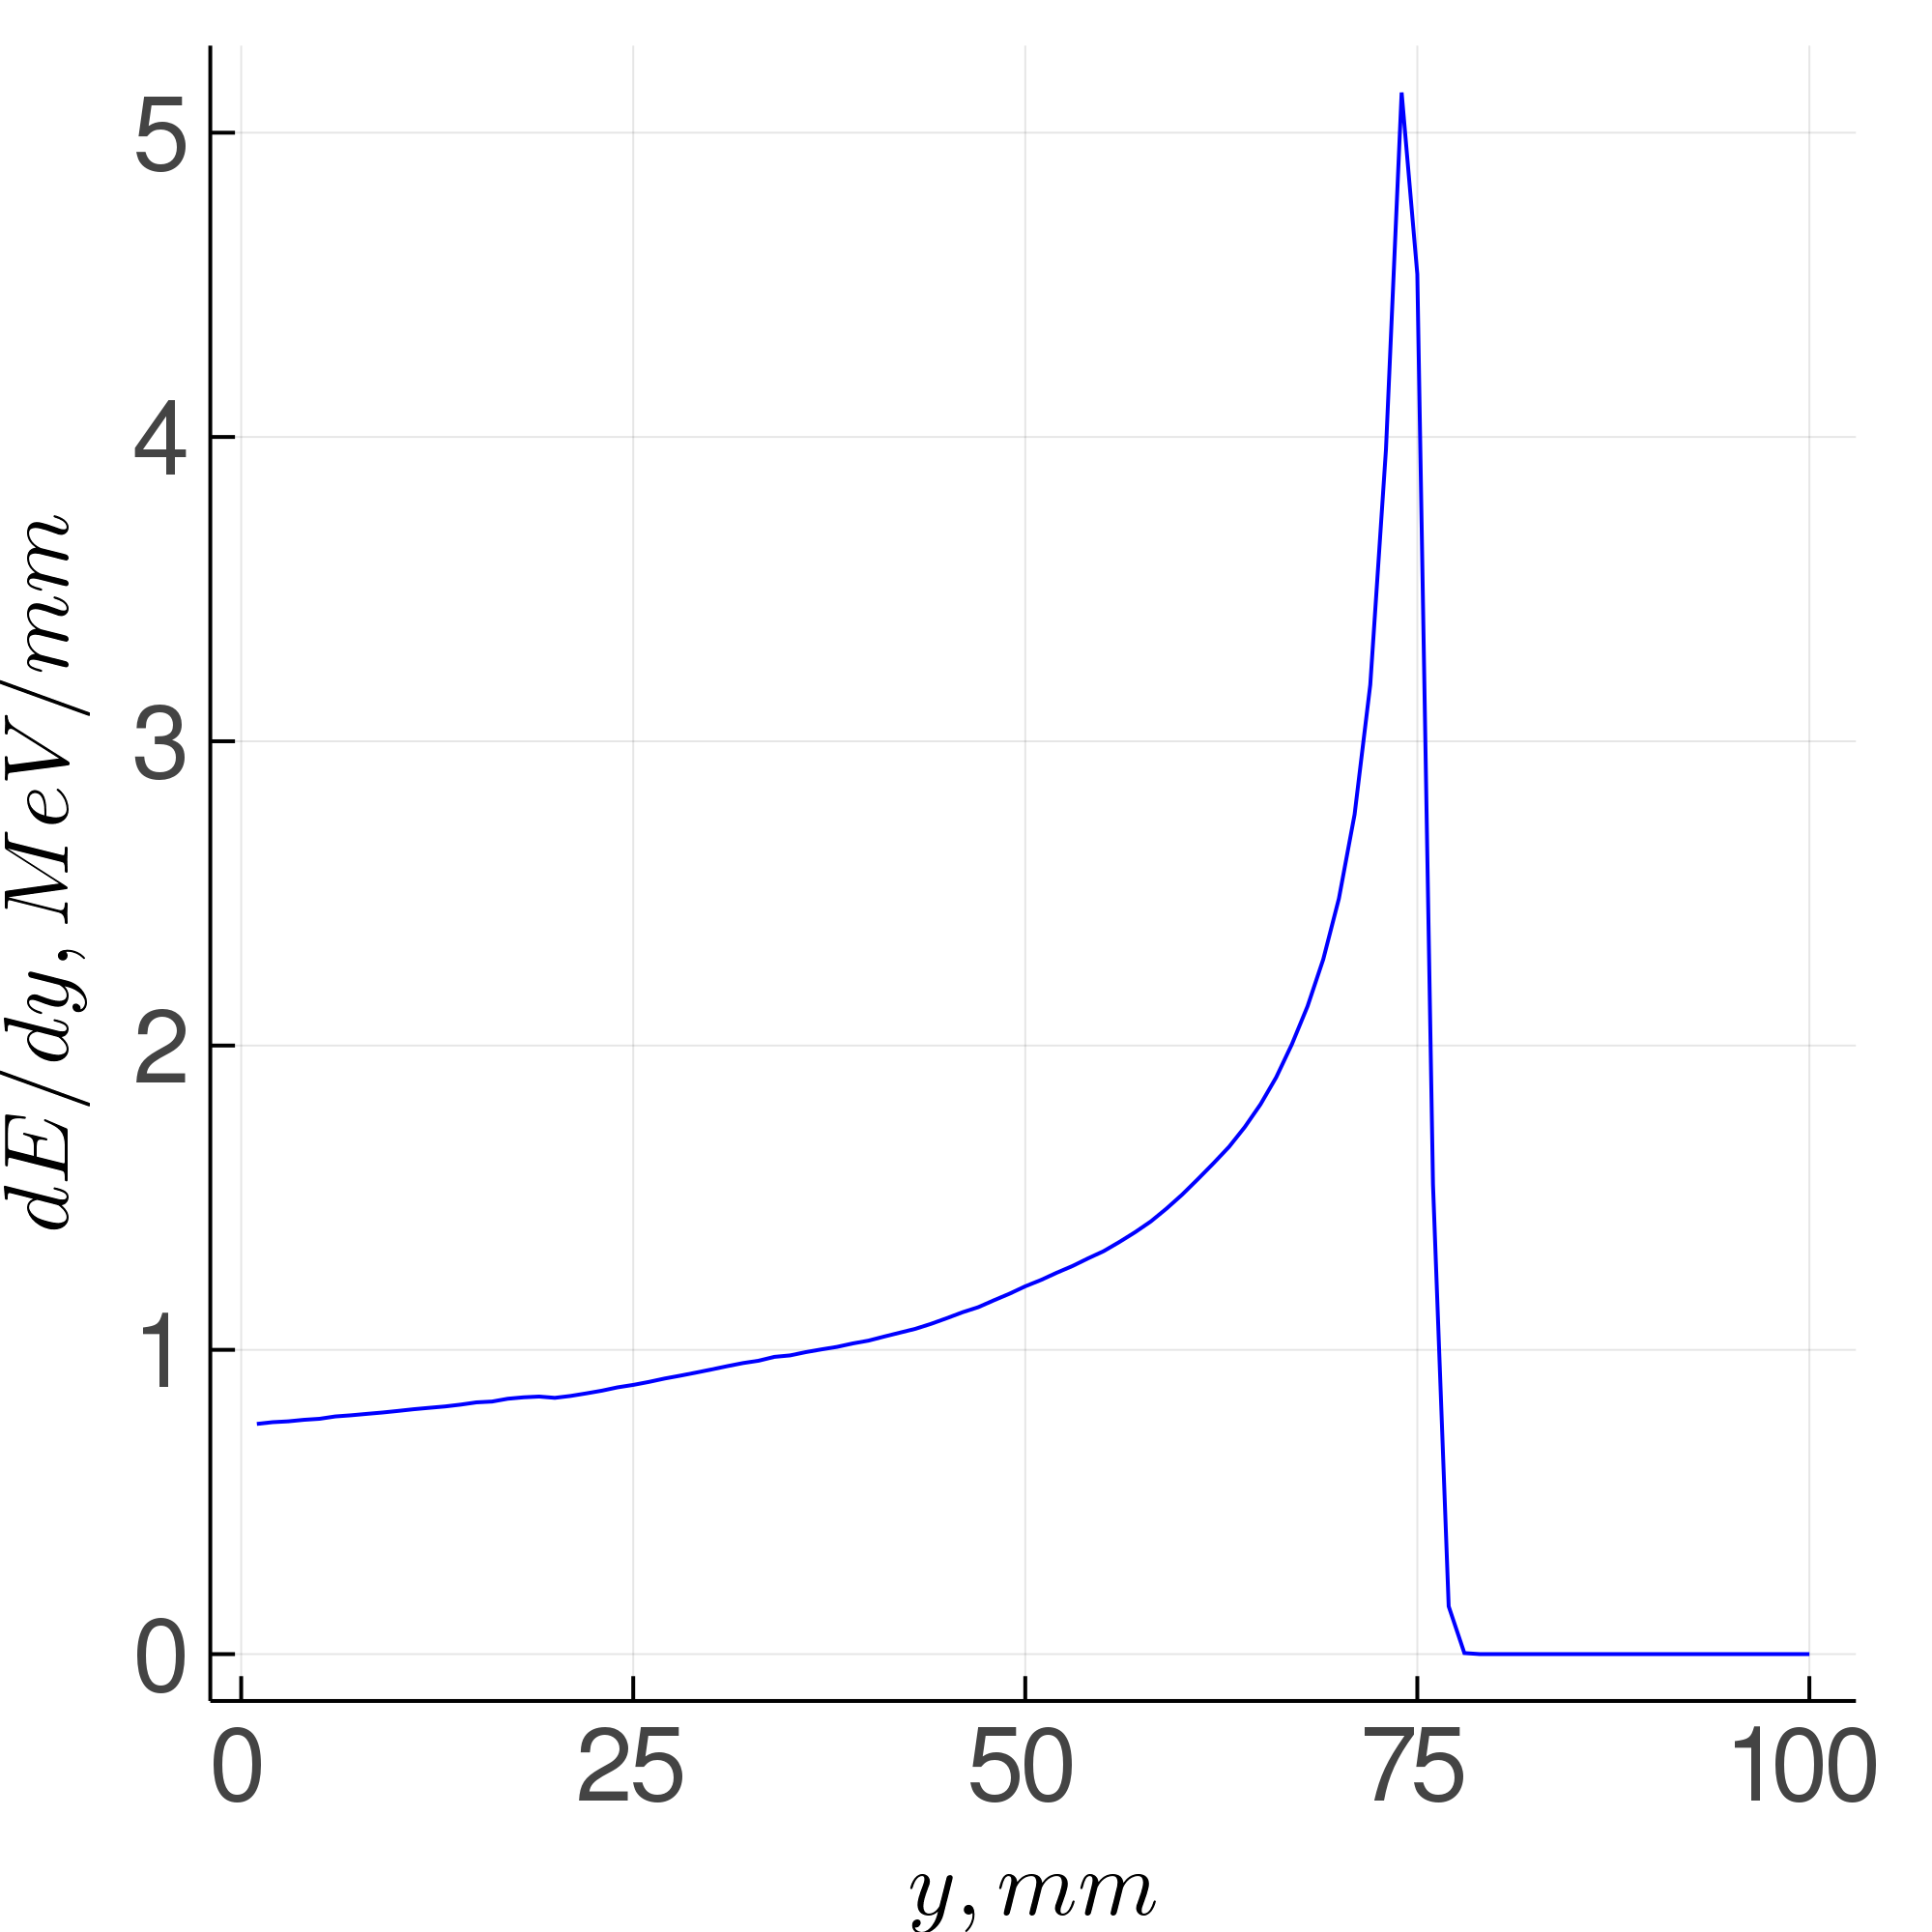
\includegraphics[width=\textwidth]{img/p_100MeV_polystirol.png}}
\caption{Кривая потерь энергии протона с энергией $E=100$ МэВ в полистироле.}
\label{p_100MeV_polystirol}
\end{minipage}
\hfill
\begin{minipage}[h]{0.5\linewidth}
\center{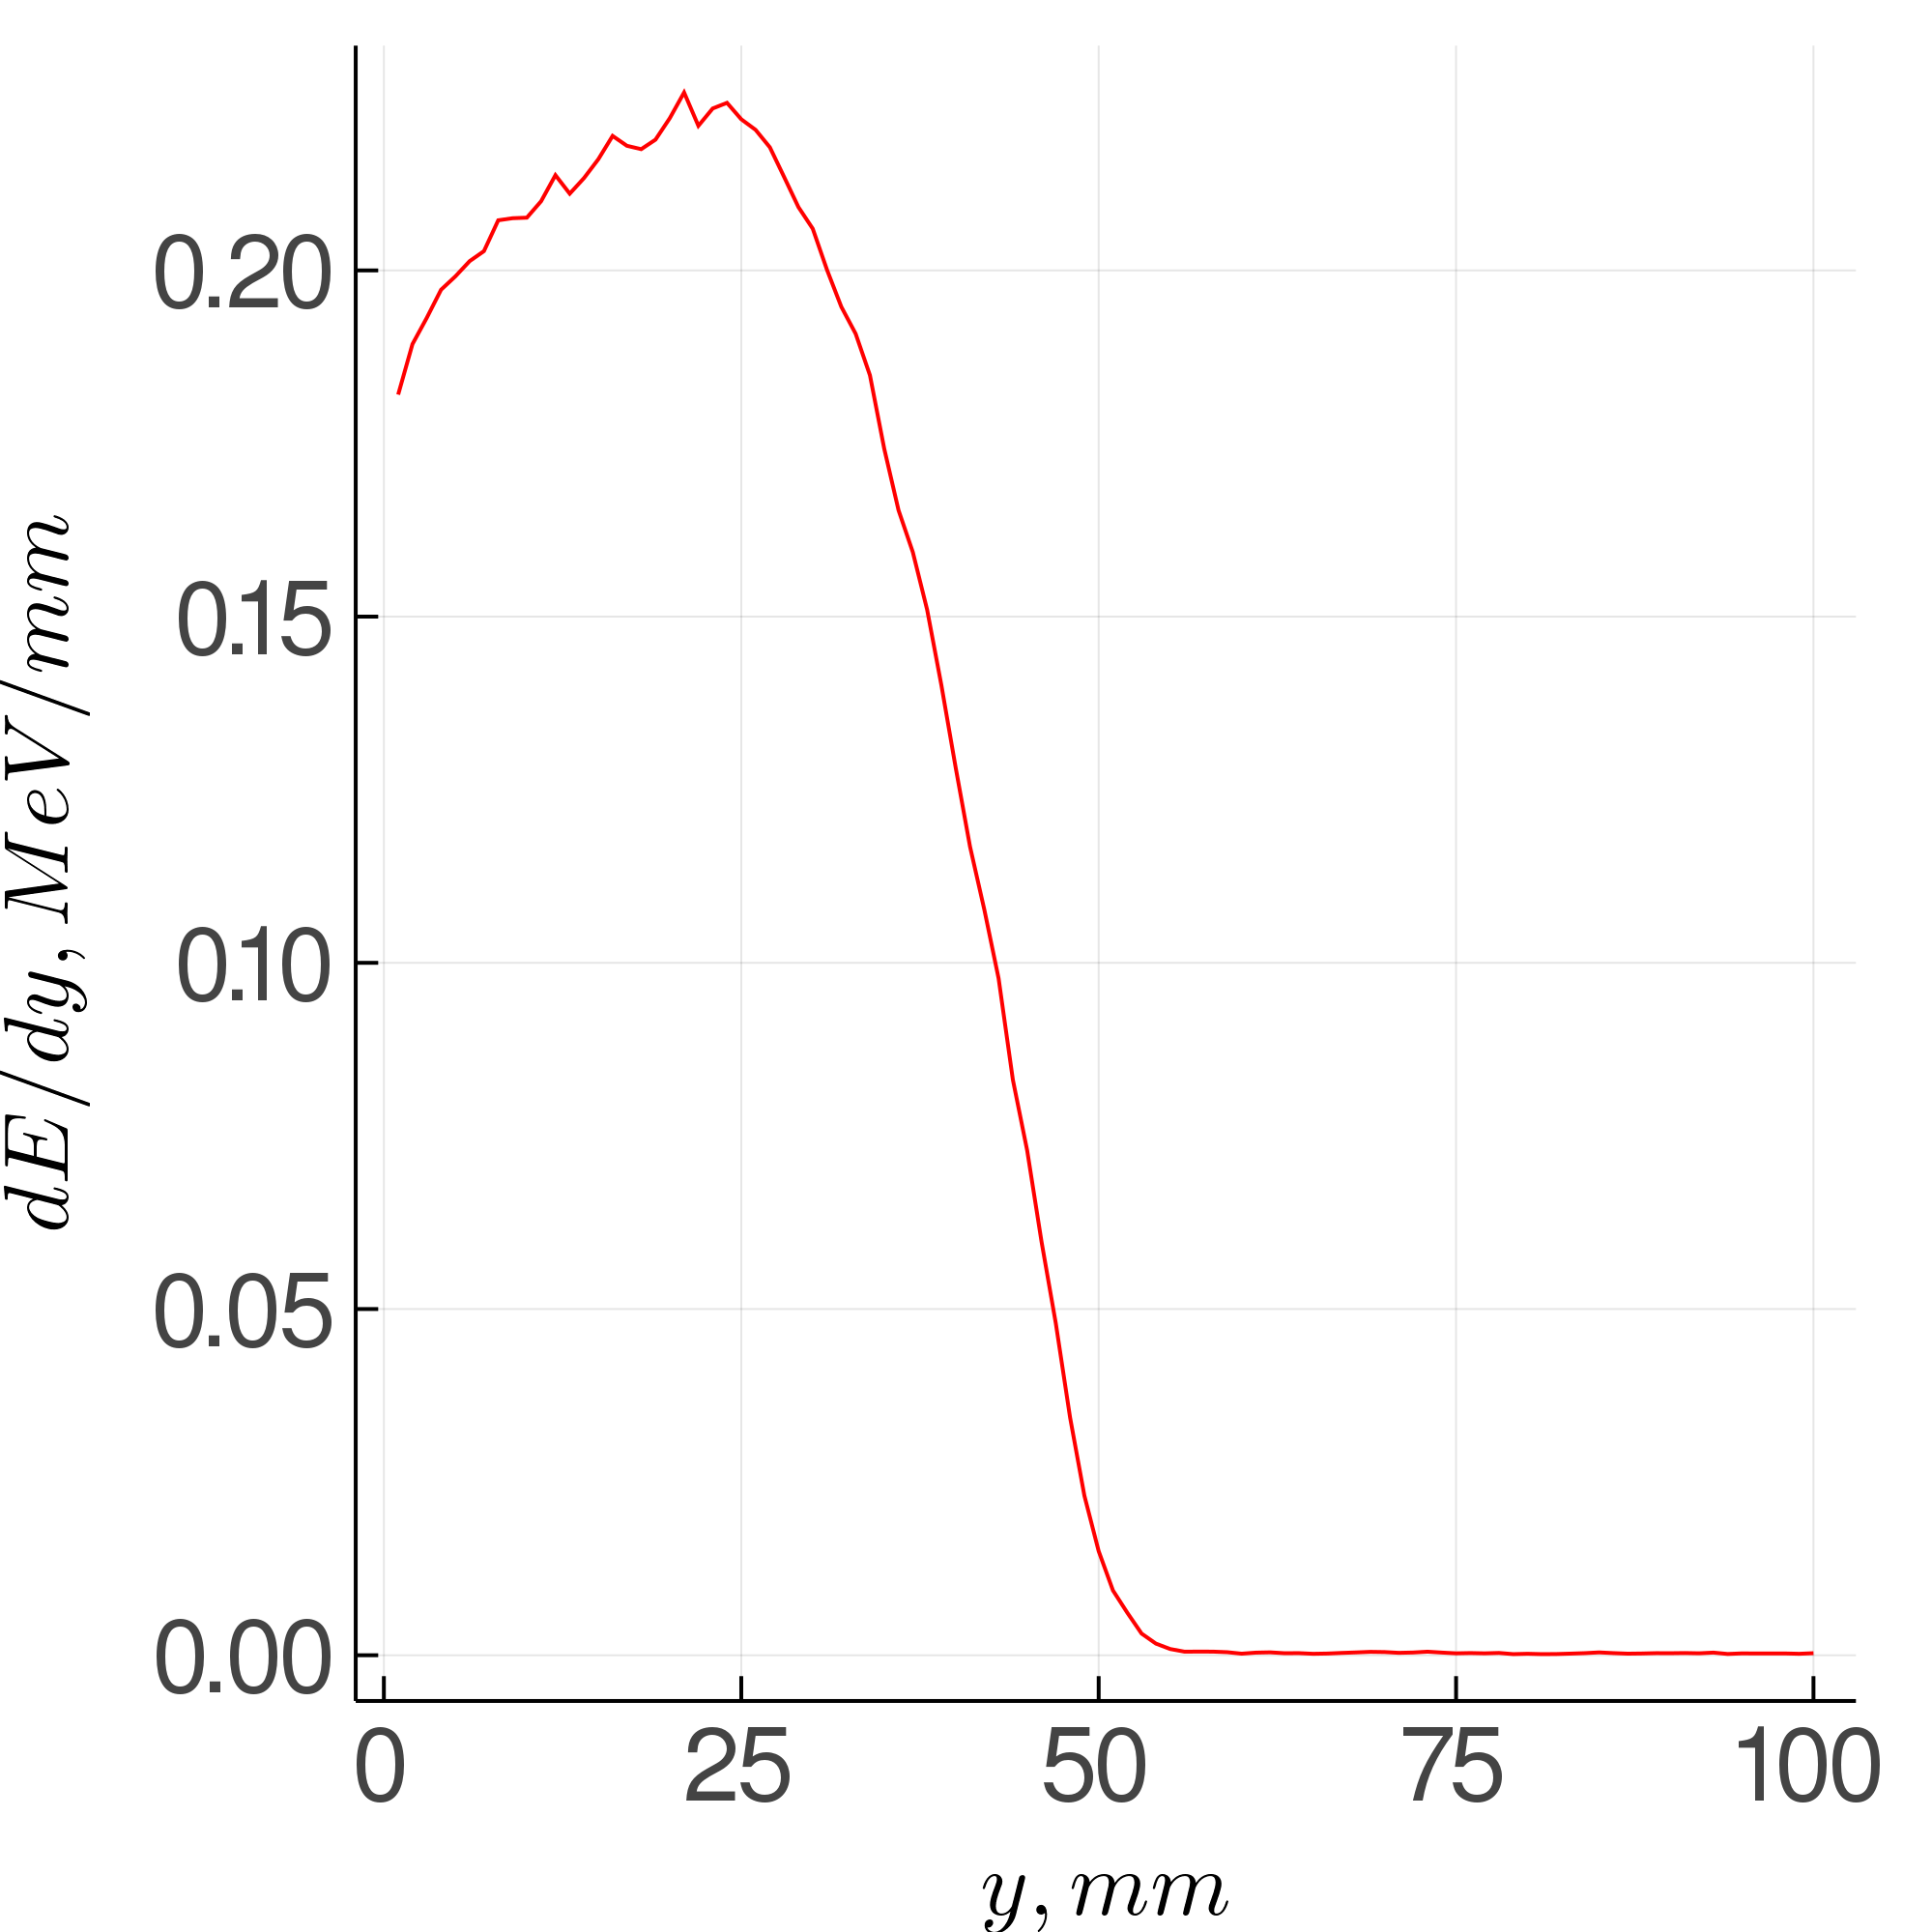
\includegraphics[width=\textwidth]{img/e_10MeV_polystirol.png}}
\caption{Кривая потерь энергии электрона с энергией $E=10$ МэВ в полистироле.}
\label{e_10MeV_polystirol}
\end{minipage}
\end{figure}

Детектор (Рис. \ref{detector}) состоит из цилиндрических сцинтилляционных шайб диаметром $2$ - $5$ см. Для того, чтобы светосбор происходил отдельно с каждой шайбы, они разделены светоотражающим материалом. Толщина шайб варьируется от $2$ до $10$ мм и может быть изменена в зависимости от удаленности шайбы от торца детектора, чтобы обеспечить лучшее разрешение. Шайбы, расположенные вблизи входного окна следует сделать тоньше, чтобы увеличить точность определения кривой потерь для электронов. Однако, утончение шайб может привести к существенному увеличению веса детектора за счет сопутствующей электроники. Полная толщина детектора выбирается с учетом минимизации его веса и с учетом диапазона энергий частиц, которые нужно регистрировать.

\begin{figure}[h!]
\center{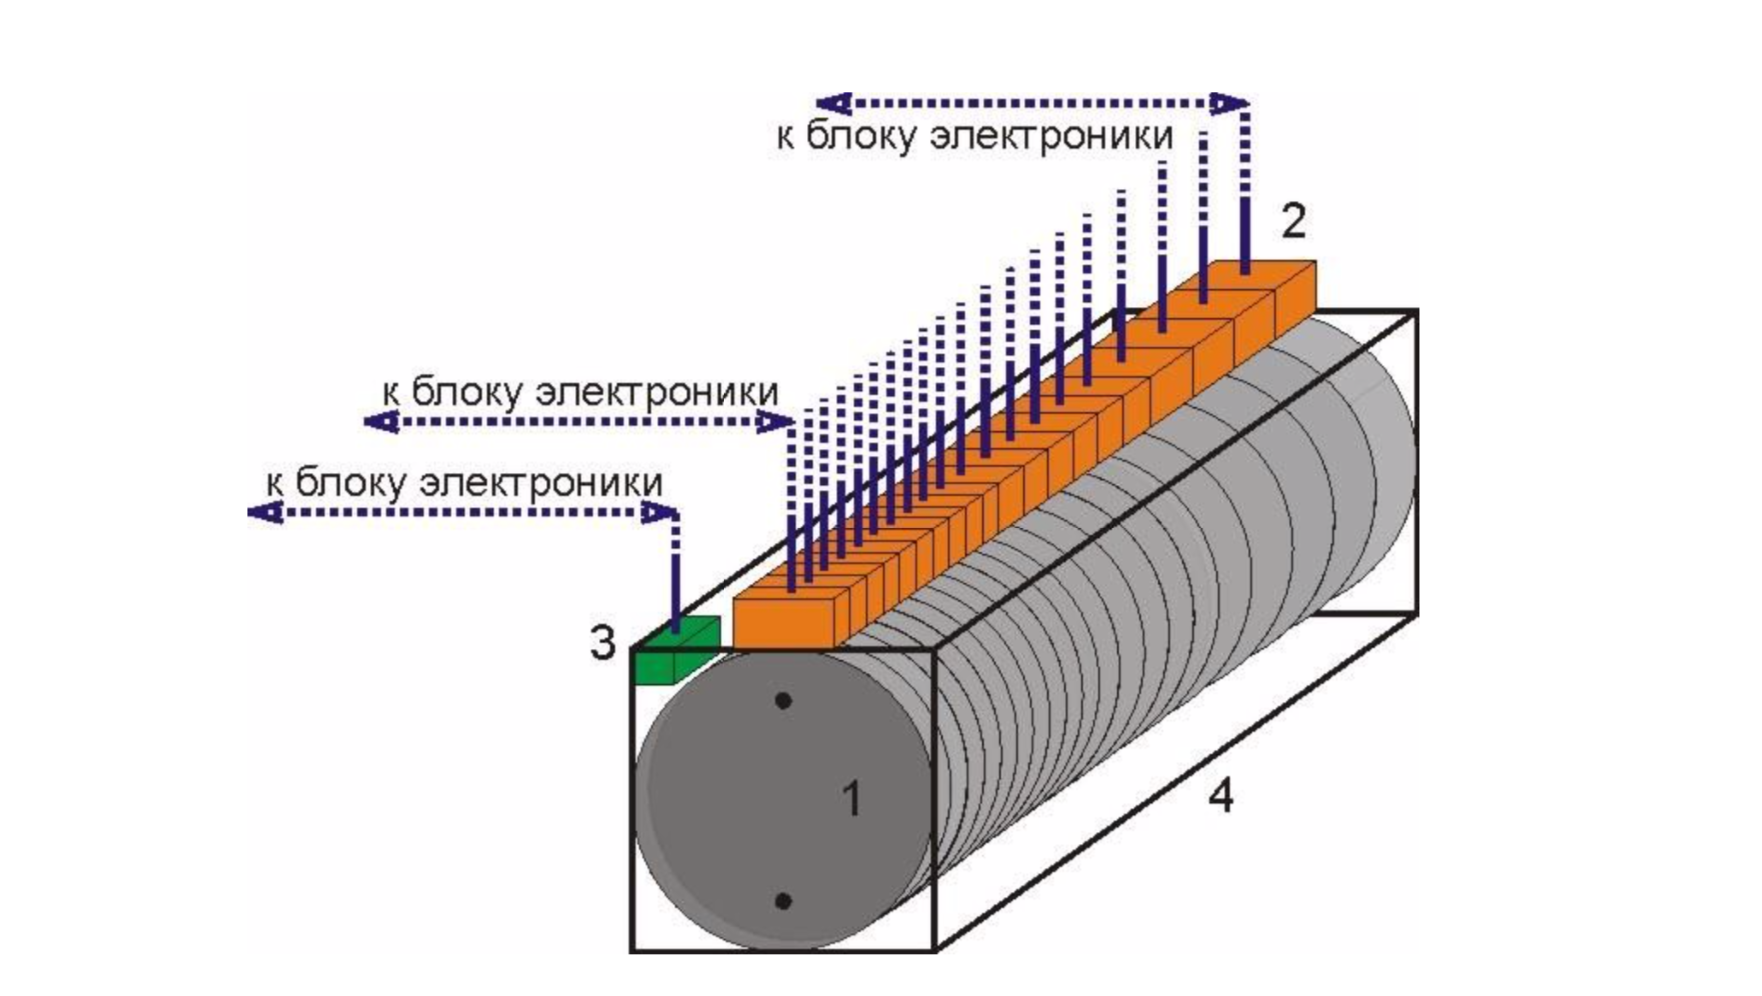
\includegraphics[width=\textwidth]{detector.png}}
\caption{Схема прототипа спутникового детектора. 1 --- сцинтилляционные шайбы, 2 --- фотоумножители, 3 --- датчик температур, 4 --- корпус детектора.}
\label{detector}
\end{figure}

Светосбор осуществляется с помощью прикрепления полупроводниковых фотоумножителей к самому сцинтиллятору или через спектросмещающее волокно.


Вся конструкция заключена в металлический корпус. Он также выполняет функцию защиты шайб от воздействия частиц, прилетающих под большим углом и обладающих малой энергией (протоны с энергией $20$ - $40$ МэВ и электроны до $4$ МэВ.). На входное окно детектора может быть установлен коллиматор или фильтр низкоэнергетичных частиц.

Детектор имеет три режима работы: дифференциальный, интегральный и смешанный. В дифференциальном режиме каждое событие анализируется отдельно, тип и энергия частицы определяются по энерговыделению в каждой шайбе. Это возможно при низкой скорости счета. В интегральном режиме происходит измерение суммарной по времени выделившейся энергии в каждой шайбе, а затем восстанавливается энергетический спектр частиц. Смешанный режим представляет собой комбинацию дифференциального и интегрального: в шайбах, близких к входному окну, происходит считывание в интегральном режиме, так как событий много, а в шайбах, расположенных далеко от входного окна, считывается каждое событие по отдельности.

Конкретные пороговые значения счета для перехода из одного режима в другой определяются свойствами сцинтиллятора, фотоумножителей и временем передачи данных.

Прототип (Рис. \ref{detector_real_2}) был собран из $20$ шайб из полистирола, каждая толщиной $4$~миллиметра и диаметром $3$~сантиметра. Шайбы соединены с фотоумножителями через спектросмещающее волокно. Такой детектор способен регистрировать протоны до $100$ МэВ и электроны до $10$ МэВ с достаточно большой точностью. Интегральный режим может быть использован начиная со скоростей счета около $1$~кГц. При скоростях счета более $100$~кГц, дифференциальный режим уже не возможно использовать.

\begin{figure}[h!]
\center{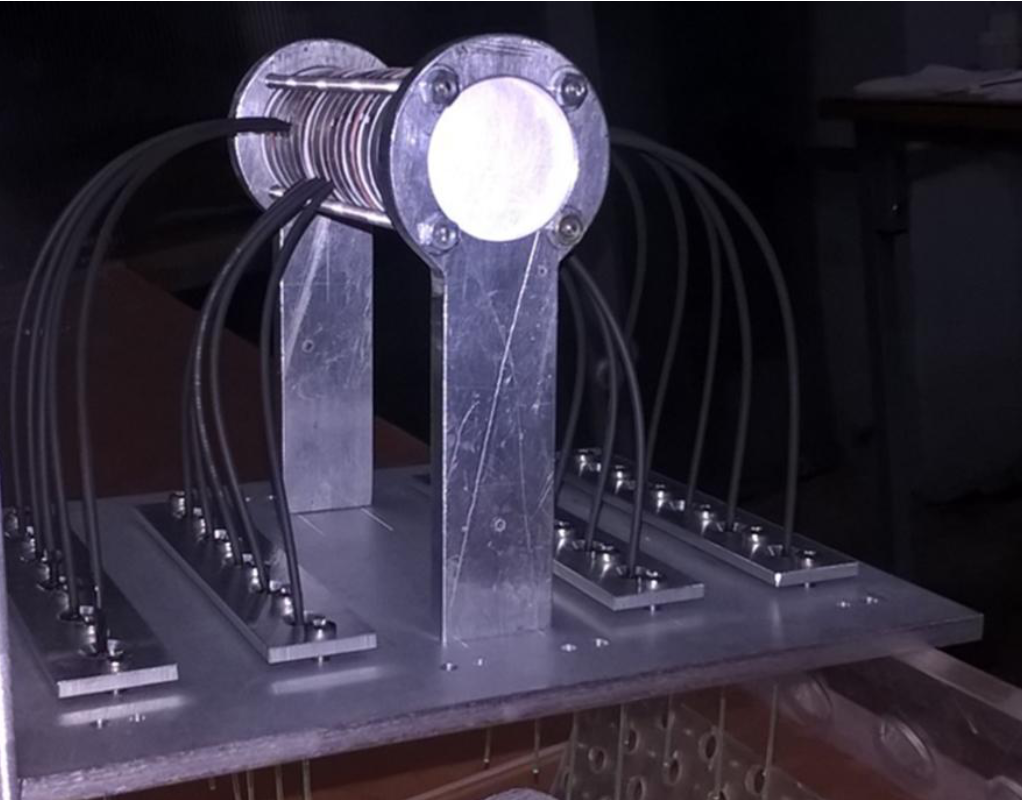
\includegraphics[width=0.6\textwidth]{detector_real_2.png}}
\caption{Фотография прототипа детектора.}
\label{detector_real_2}
\end{figure}

Ожидаемый спектр протонов и электронов, который можно наблюдать при событиях солнечной активности \cite{real_energy_spectrum} показывает, что без интегрального режима обойтись нельзя: поток частиц с относительно низкой энергией превышает ограничение, обусловленное временем обработки сигнала детектором (Рис. \ref{electrons_real_spectrum}, \ref{protons_real_specrtum}).

\begin{figure}[h]
\begin{minipage}[h]{0.5\linewidth}
\center{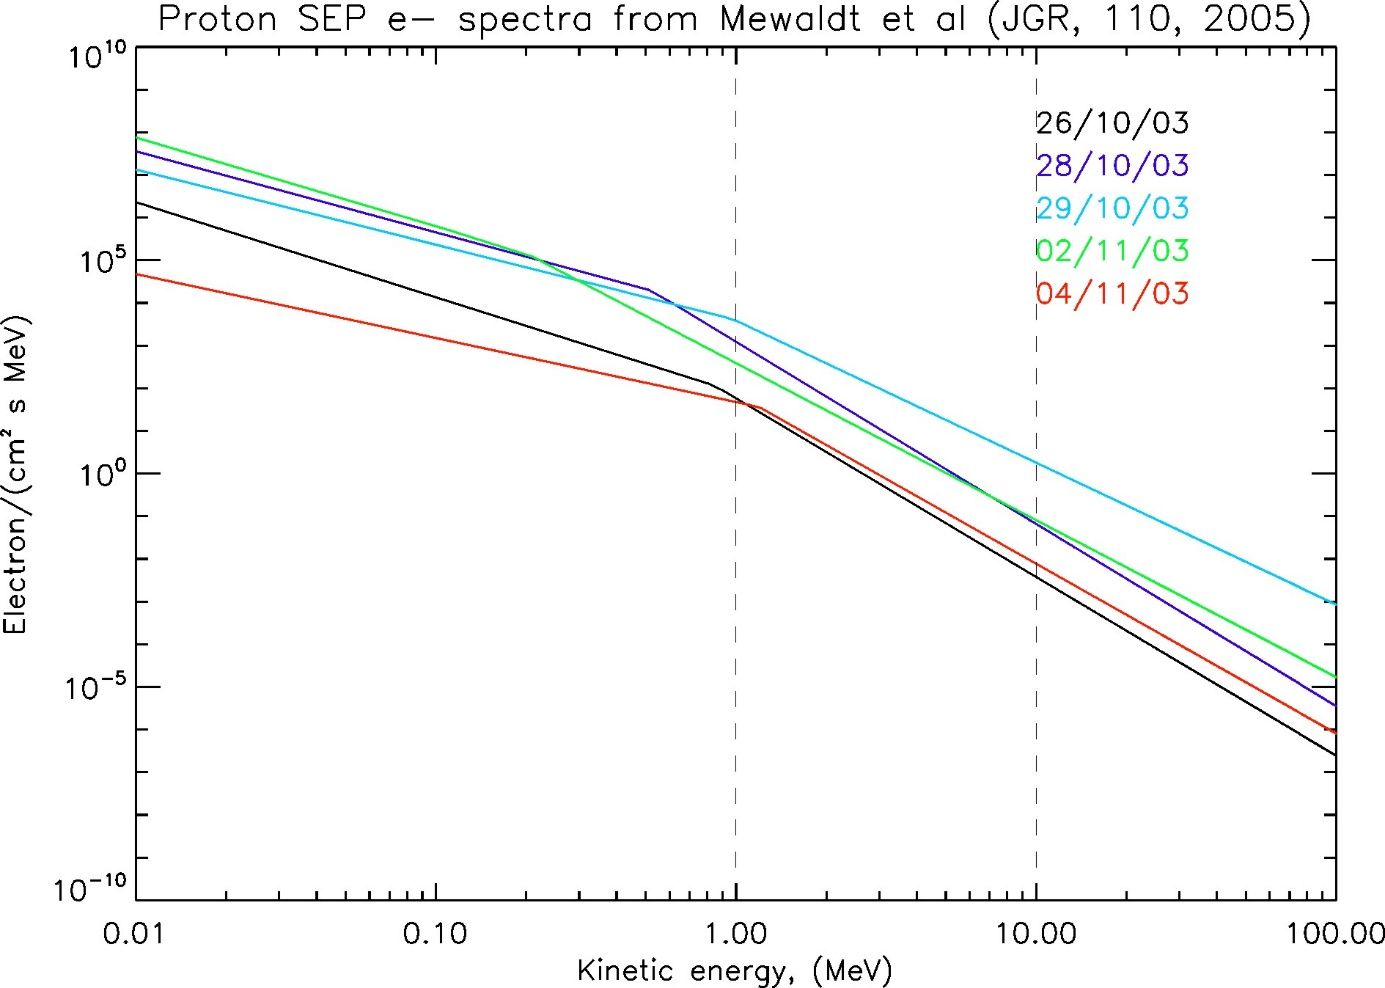
\includegraphics[width=0.95\textwidth]{img/electrons_real_spectrum.png}}
\caption{Спектр электронов во время событий солнечной активности 2003г \cite{real_energy_spectrum}.}
\label{electrons_real_spectrum}
\end{minipage}
\hfill
\begin{minipage}[h]{0.5\linewidth}
\center{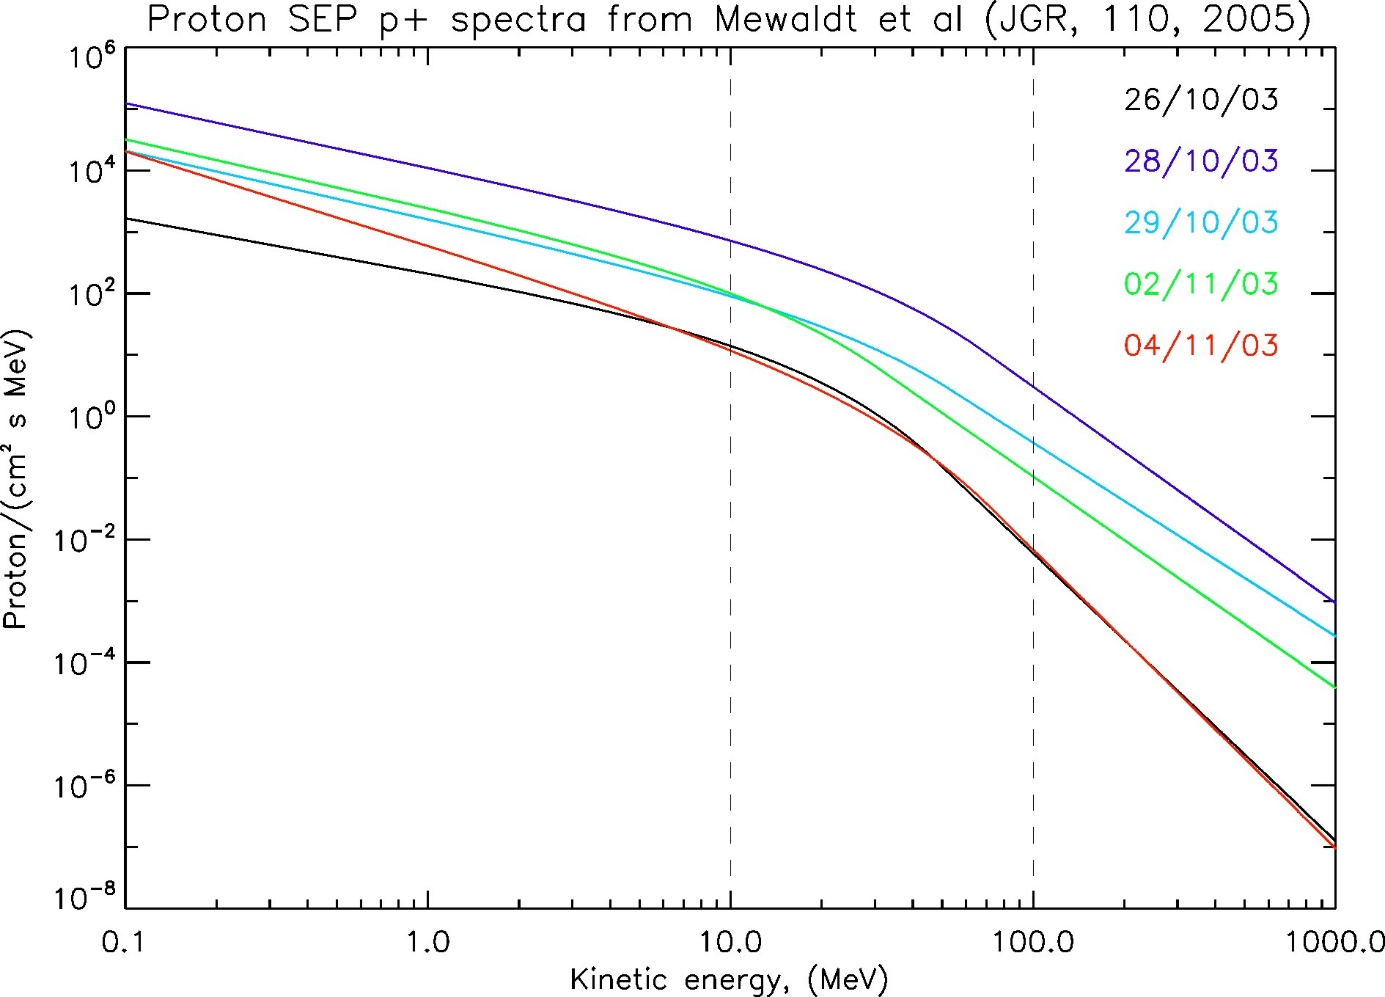
\includegraphics[width=0.95\textwidth]{img/protons_real_specrtum.png}}
\caption{Спектр протонов во время событий солнечной активности 2003г.}
\label{protons_real_specrtum}
\end{minipage}
\end{figure}


\clearpage

\section{Восстановление спектров}

\subsection{Данные}

~~~~В настоящее время реальные данные для этого эксперимента еще не набраны, поэтому в данной работе описывается методика обработки и ее тестирование на смоделированных данных.

Моделирование спектров проводилось с помощью Geant4 \cite{geant4}. Geant4 - библиотека, написанная на языке программирования C++, которая позволяет моделировать физические процессы с помощью Монте-Карло методов.

В качестве модельных данных использовались результаты Geant4 модели  детектора из 100 шайб диаметрой 3 сантиметра и толщиной 1 миллиметр из полистирола. Было смоделировано прохождение протонов через с энергиями от 1 до 150 МэВ с шагом 1 МэВ, имеющих следующие распределения по углам:
\begin{itemize}
    \item В одном направлении, перпендикулярно шайбам
    \item С нормальным распределением по углу со средним значением $\mu = 0^\circ$ и дисперсией $\sigma=5^\circ$
    \item С равномерным распределением по углу от $0^\circ$ до $15^\circ$
\end{itemize}

\subsection{Постановка задачи}
~~~~В реальном эксперименте при работе детектора в интегральном режиме будет измеряться суммарное за некоторый промежуток времени $t$ энерговыделение в каждой n-той шайбе $\{f_n\}_{n=1}^N$ с некоторыми ошибками измерения $\{\delta f_n\}_{n=1}^N$ (либо с матрицей корелляций $\Sigma$). Будем считать, что за время проведения измерения поток частиц остается примерно постоянным, то есть что $t$ много меньше характерного времени изменения потока и проводимое измерение имеет смысл. Предположим, что частицы могут иметь энергию от $E_{min}$ до $E_{max}$.

Для того, чтобы из этих данных получить спектр протонов, нужно понять, какой отклик дает протон с энергией $E$ в шайбе под номером $n$, то есть прокалибровать детектор. Обозначим эту величину $K(E, n)$. Прокалибруем детектор на протонах с энергиями $\{E_l\}_{l=1}^L$, охватывающими диапазон от $E_{min}$ до $E_{max}$. Для произвольной энергии $E$ будем считать, что:

\begin{equation}
    K(E, n) = \frac{K(\varepsilon_{min}, n) \cdot (\varepsilon_{max} - E) + K(\varepsilon_{max}, n) \cdot (E - \varepsilon_{min})}{\varepsilon_{max} - \varepsilon_{min}},
\end{equation}

\begin{equation}
    \varepsilon_{min} = \max(\varepsilon \text{: } \epsilon \in \{E_l\}_{l=1}^L \text{, } \varepsilon \leq E),
\end{equation}
\begin{equation}
    \varepsilon_{max} = \min(\varepsilon \text{: } \varepsilon \in \{E_l\}_{l=1}^L \text{, } \varepsilon \geq E),
\end{equation}
то есть сделаем линейное приближение.


Обозначим искомый спектр как $\varphi(E)$. Тогда
\begin{equation}
    f_n = \int_{E_{min}}^{E_{max}} K(E, n) \varphi(E) dE,
\end{equation}

Далее будем рассматривать различные способы решения этой задачи.

\subsection{Различные методы восстановления}

~~~~Разложим функцию $\varphi(E)$ по базису $\{T_m(E)\}_{m=1}^M$, коэффициенты разложения обозначим как $\{\varphi_m\}_{m=1}^M$:
\begin{equation}
    \varphi(E) = \sum_{m=1}^M \varphi_m T_m(E)
\end{equation}
Также определим матрицу $K_{mn}$ от функции отклика $K(E, n)$ :
\begin{equation}
    K_{mn} = \int_{E_{min}}^{E_{max}} K(E, n) T_m(E) dE
\end{equation}
Тогда задача сводится к решению матричного уравнения относительно $\varphi_m$
\begin{equation} \label{matrix_eq}
    f_n = K_{mn} \varphi_m
\end{equation}
Существует множество методов восстановления спектров в поставленной задаче:
\begin{enumerate}
    \item Напрямую решить уравнение (\ref{matrix_eq}). Из-за плохой обусловленности матрицы малые ошибки в $f$ приведут к большим ошибкам в $\varphi$
    \item Для каждой базисной функции построить отклик детектора $F_i(x) = f(T_i(E))$, попробовать получить разложение $f$ по базису функций ${F_i}$, что по сути эквивалентно решению матричного уравнения
    \item Использовать преобразование Фурье: при $K(t, x) = K(t - x)$ и интегрировании по всей действительной прямой результирующая функция представляет собой свертку ядра и искомой функции. Таким образом, искомую функцию можно найти с помощью прямого и обратного преобразований Фурье. Но этот метод накладывает условия на параметры задачи.
    
    \item Воспользоваться методом статистической регуляризации (будет описан далее)
\end{enumerate}
и множество других вариантов. В данной работе подробнее остановимся на применении статистическом регуляризации Турчина c некоторыми модификациями.

\subsection{Статистическая регуляризация Турчина}
~~~~Будем искать решение уравнения (\ref{matrix_eq}) как
\begin{equation}
    \vec{\varphi}_{opt} = E[\vec{\varphi} | \vec{f}] = \int \vec{\varphi} P(\vec{\varphi} | \vec{f}) d \vec{\varphi}
\end{equation}
По формуле Байеса:
\begin{equation}
    P(\vec{\varphi} | \vec{f}) = \frac{P(\vec{\varphi})P(\vec{f} | \vec{\varphi})}{\int d \vec{\varphi} P(\vec{\varphi})P(\vec{f} | \vec{\varphi})}
\end{equation}

\subsubsection{Априорная информация}
~~~~В качестве априорной информации $P(\varphi)$ может быть использовано любое распределение. Например, будем использовать информацию о том, что искомая функция является относительно гладкой. Введем матрицу средних значений вторых производных
\begin{equation}
    \Omega_{ij} = \int_{E_{min}}^{E_{max}}\frac{d^2 T_i(x)}{dx^2} \frac{d^2 T_j(x)}{dx^2} dx
\end{equation}
Параметризуем гладкость некоторым параметром $\alpha$
\begin{equation}
    \alpha \int (\vec{\varphi}, \Omega \vec{\varphi})P(\vec{\varphi}) d \vec{\varphi} = 1
\end{equation}
и потребуем, чтобы это условие привносило как можно меньшую информацию о решении, то есть информационная энтропия имеет минимальное значение
\begin{equation}
    \int P(\vec{\varphi})\ln{P(\vec{\varphi})} d \vec{\varphi} \rightarrow \min{}
\end{equation}
Решением этой задачи является параметрически заданное распределение (Приложение 1.)
\begin{equation}
    P(\vec{\varphi}) \sim \exp{-\frac{1}{2} (\vec{\varphi}, \alpha \Omega \vec{\varphi})}
\end{equation}
Выбор параметра регуляризации $\alpha$ может быть произвольным, например:
\begin{itemize}
    \item Вручную
    \item Усреднение по всем значениям параметра:
    \begin{equation}
        P(\vec{\varphi}) = \int P_{\alpha}(\vec{\varphi}) d \alpha
    \end{equation}
    \item Выбрать наиболее вероятный:
    \begin{equation}
        P(\vec{\varphi}) = P_{\alpha^*}(\vec{\varphi})
    \end{equation}
    \begin{equation}
        \alpha^* = \underset{\alpha}{\arg\max}(P(\alpha | \vec{f}))
    \end{equation}
\end{itemize}
При этом только усреднение по всем возможным параметрам $\alpha$ является объективной оценкой априоного распределения.

\subsubsection{Распределение измеренной величины}
Измеренная величина $\vec{f}$ может иметь любое распределение, но чаще всего распределена нормально. С учетом ее среднего значения и ошибок получим:
\begin{equation}
    P(\vec{f} | \varphi) = \frac{1}{(2\pi)^{N/2} \sqrt{\det{\Sigma}}}\exp{-\frac{1}{2}(\vec{f} - K \vec{\varphi})^T \Sigma^{-1} (\vec{f} - K \vec{\varphi})}
\end{equation}
Заметим, что произведение априорного распределения и распределения измеренной величины имеет вид многомерного нормального распределения. Тогда оптимальное значение вектора $\vec{\varphi}$ и матрицу ковариаций можно вычислить аналитически, так как для многомерного нормального распределения матожидание и дисперсионную матрицу можно получить не поиском моды, а просто из вида самого распределения (Приложение 2.).
\begin{equation}
    \vec{\varphi}_{opt} = (K^T \Sigma^{-1}K + \alpha \Omega)^{-1} K^T \Sigma^{-1T} \vec{f}
\end{equation}
Так же легко найти матрицу ковариаций
\begin{equation}
    cov = (K^T \Sigma^{-1} K + \alpha \Omega)^{-1}
\end{equation}

Если величина $\vec{f}$ имеет распределение, отличное от нормального, то аналитическое решение не всегда легко найти. Тогда стоит задача поиска моды или матожидания и дисперсии произвольного апостериорного распределения. С учетом того, что оптимальная размерность базиса пространства восстановления функции составляет примерно 20-30 измерений, поиск необходимых параметров не может быть осуществлен с помощью градиентных и сеточных методов, нужно использовать методы Монте-Карло \cite{montecarlo_simple}.

\subsubsection{Решение}
Получив коэффициенты разложения по базису и матрицу ковариаций этого вектора, можно найти значение функции спектра в любой точке, лежащей между $E_{min}$ и $E_{max}$:
\begin{equation}
    \varphi(E) = \sum_{m=1}^M \varphi_m T_m(E)
\end{equation}
и ошибку вычисления спектра в этой точке:
\begin{equation}
    \delta \varphi(E) = \sqrt{\vec{T}^T(E) \cdot cov \cdot \vec{T}(E)},
\end{equation}
где $\vec{T}(E)$ - вектор значений базисных функций в точке $E$.
\subsection{Язык программирования Julia}
~~~~Для реализации алгоритма статистической регуляризации был использован язык программирования Julia.

Он имеет высокую производительность, допускает параллельное исполнение кода, позволяет легко выразить множество объектно-ориентированных и функциональных шаблонов программирования. Язык достаточно прост для изучения,  имеет высокоуровневый синтаксис и динамическую типизацию. Помимо этого, язык хорошо подходит для обработки данных, так как существует множество математических и графических библиотек, написанных на Julia. Julia позволяет вызывать функции, написанные на других языках программирования. Существует множество пакетов, генерирующих выборку из заданного распределения. Одним из самых удобных из них является BAT.jl \cite{bat}. Он использует классические алгоритмы МСМС и прост в применении. Язык был выбран в частности для того, чтобы обеспечить легкую совместимость с этим пакетом.


\subsection{TurchinReg.jl}
~~~~Далее опишем содержание написанного пакета \href{https://github.com/mipt-npm/TurchinReg.jl}{TurchinReg.jl}.

\subsubsection{Базисы}
~~~~Для начала нужно выбрать базис для восстанавливаемой функции. Выбор базиса значительно влияет на восстановление. Например, если все функции базиса принимают на правом конце отрезка нулевое значение, то их любая комбинация, а вследствие и найденная функция, будет иметь на правом конце нулевое значение. Поэтому базис нужно выбирать исходя из ожидаемого спектра. В пакете реализованы 4 базиса (подробное описание в Приложении 3):
\begin{enumerate}
    \item Фурье-базис
    \item Кубические сплайны
    \item Полиномы Лежандра
    \item Полиномы Бернштейна
\end{enumerate}

Самым универсальным является базис из кубических сплайнов, потому что он не содержит полиномов большой степени (следовательно, позволяет использовать большие размерности, не вызывая вычислительных проблем) и хорошо описывает произвольную гладкую функцию.

Также есть возможность создать свой собственный базис, определив отрезок, вид базисных функций и матрицу средних значений вторых производных.

\subsubsection{Распределение измеренной случайной величины}
~~~~В зависимости от распределения $\vec{f}$, можно выбрать решение аналитическим методом или с помощью Монте-Карло методов. Генерировать выборки из нужного распределения можно с помощью трех пакетов:
\begin{enumerate}
    \item BAT.jl
    \item AHMC.jl
    \item DHMC.jl
\end{enumerate}
В первом реализован классический алгоритм Метрополиса-Хастингса \cite{metropolis}. Во втором и третьем пакетах используются гамильнотовы методы Монте-Карло \cite{hamiltonian_mc}, которые дают большую точность и меньшее время генерации выборки. Причем наличие у апостериорного распределения только одном моды не гарантируется, поэтому нужно учитывать возможную мультимодальность распределения при генерации выборки. Для решения проблемы многомодальных распределений можно использовать ограничения на коэффициенты, которые будут рассмотрены далее.

\subsubsection{Выбор параметра регуляризации}
С точки зрения статистики, наилучшим методом является интегрирование по всем параметрам регуляризации $\alpha$, которое может быть проведено с помощью Монте-Карло методов. Предполагая, что у значения параметра есть максимум, и он является достаточно узким, можно заменить распределение по параметру гладкости на дельта-функцию и избежать использования Монте-Карло интегрирования в при нахождении параметра гладкости. Тогда в задаче с гауссовым распределением $\vec{f}$ получим полностью аналитическое решение. Также можно указать произвольное значение параметра регуляризации вручную.

\subsubsection{Ограничение на значение компонент вектора}
~~~~В физических задачах функция часто имеет только численные ограничения. Например, число событий не может быть отрицательным. Чтобы учесть это в восстановлении, нужно уменьшить апостериорную вероятность физически неверных значений. Существует два способа поставить ограничения: либо на компоненты вектора $\vec{\varphi}$, например, $0 < \varphi_i < 10$, либо на значение функции в наборе точек $\{E_i\}_{i=1}^I$, например, $0 < \sum_{m=1}^M \varphi(E_i) T_m(E_i) < 10$.

Строгие границы параметров часто вызывают вычислительные проблемы, поэтому будем домножать исходную вероятность на затухающую экспоненту при достижении параметром левой или правой границы. Пусть $\vec{\varphi}_{min}$ --- левая граница,  $\vec{\varphi}_{max}$ - правая граница, $\vec{\varphi}_0$ --- коэффициенты нормировки отклонения от границы, $I(x)$ - индикатор события $x$.
\begin{equation}
    C_{lower} = \sum_{m=1}^M I(\varphi_m < \varphi_{min\text{ }m}) \cdot \frac{\varphi_{min\text{ }m} - \varphi_m}{\varphi_{0 m}}
\end{equation}
\begin{equation}
    C_{higher} = \sum_{m=1}^M I(\varphi_m > \varphi_{max\text{ }m}) \cdot \frac{\varphi_{m} - \varphi_{max\text{ }m}}{\varphi_{0 m}}
\end{equation}
\begin{equation}
    P(\varphi | f)_{\varphi_{min} <\varphi < \varphi_{max}}  = P(\varphi | f) \cdot
e^{- C_{lower}} \cdot e^{- C_{higher}}
\end{equation}

Аналогично можно ввести ограничение на значение функции в наборе точек.

\subsection{Обработка данных}
~~~~В качестве ожидаемого спектра было взято одно из событий солнечной активности, описанное в \cite{real_energy_spectrum} (Рис. \ref{real_spectrum_plot}).

\begin{figure}[h!]
    \center{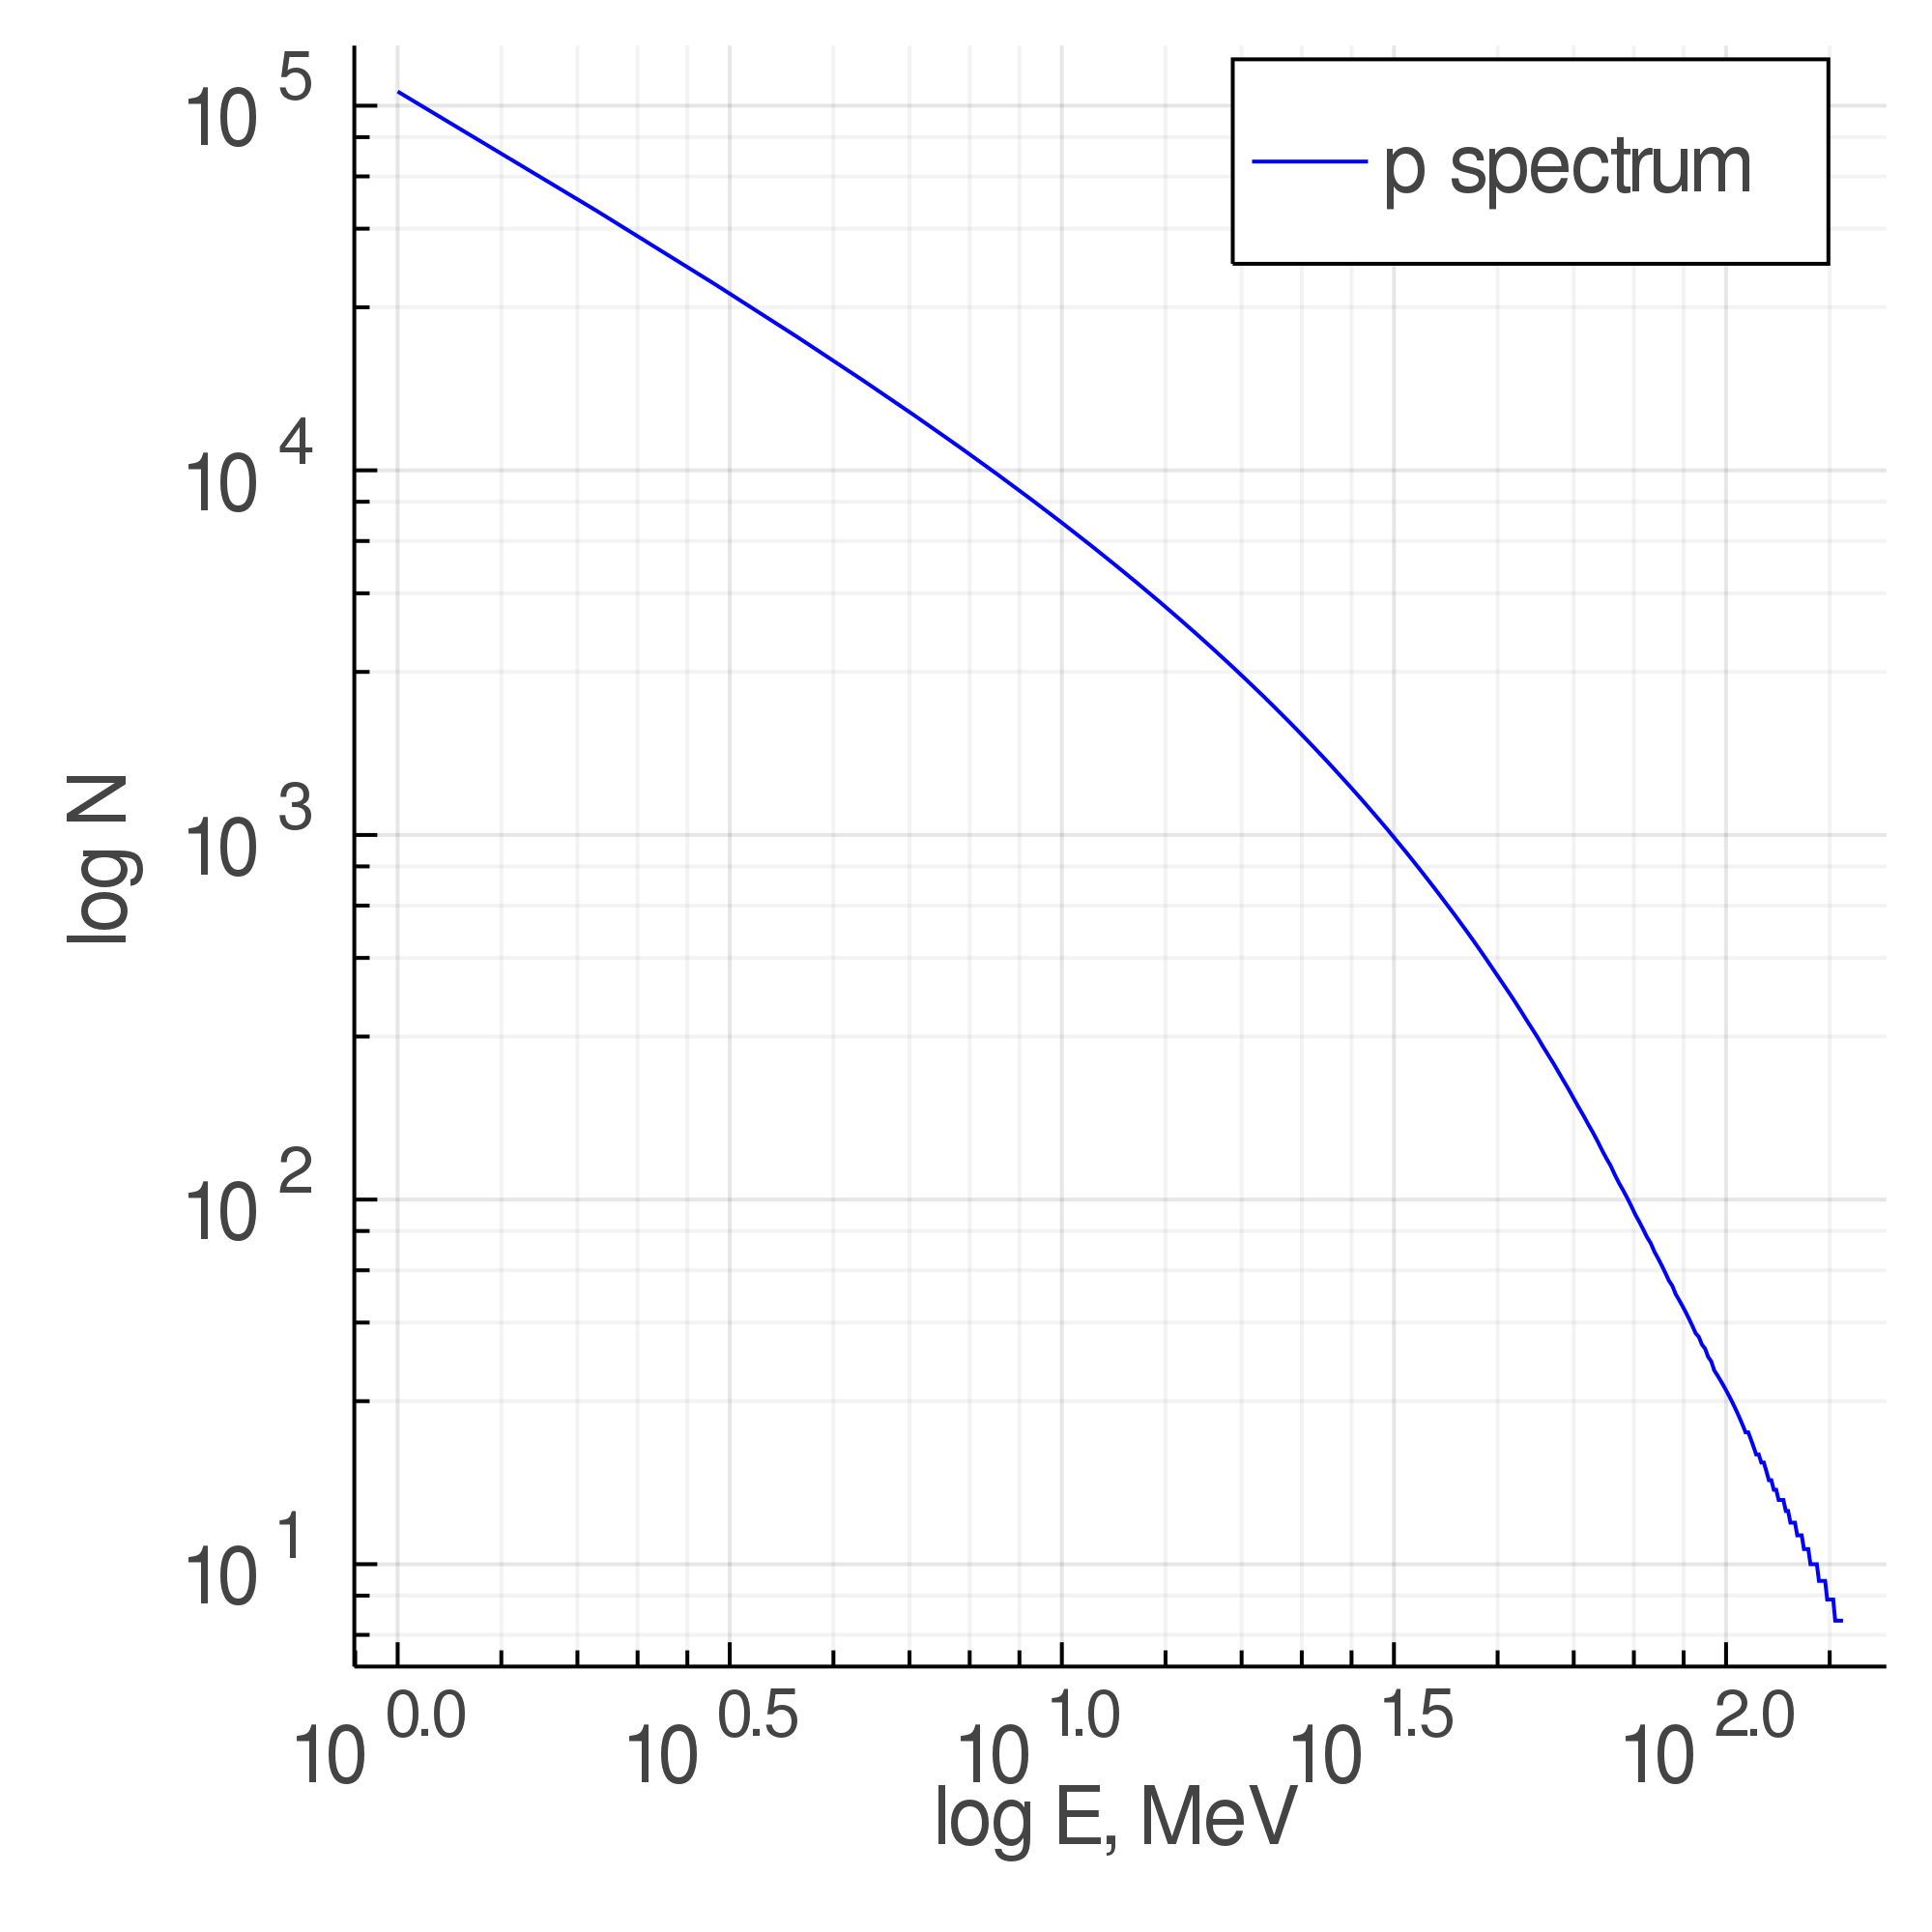
\includegraphics[width=0.6\textwidth]{new_pic/p_spectrum.png}}
    \caption{Ожидаемый спектр.}
    \label{real_spectrum_plot}
\end{figure}


Рассматриваются два случая:
\begin{itemize}
    \item 100 шайб по 1 мм
    \item 25 шайб по 4 мм
\end{itemize}
Второй случай реализуется с помощью суммирования энерговыделения в каждых четырех подряд идущих шайбах и больше соответствует реальной конструкции детектора.

Изначально есть некоторый набор смоделированных данных, из которого можно построить калибровочные кривые $kernel(E, n)$ (Рис. \ref{K}, \ref{K_25}) и отклик детектора $f(n)$ в некотором наборе точек $measurement\_points$.
Функция отклика детектора $kernel$ аппроксимируется по калибровке по энергиям ${E_i}$ как
\begin{equation}
    K(E, n) = \frac{kernel(E_{lower}, y) (E_{higher} - E) + kernel(E_{higher}, y) (E - E_{lower})}{E_{higher} - E_{lower}}
\end{equation}
где $E_{lower} \leq E < E_{higher}$, $E \in {E_i}$.


\begin{figure}[h]
\begin{minipage}[h]{0.45\linewidth}
\center{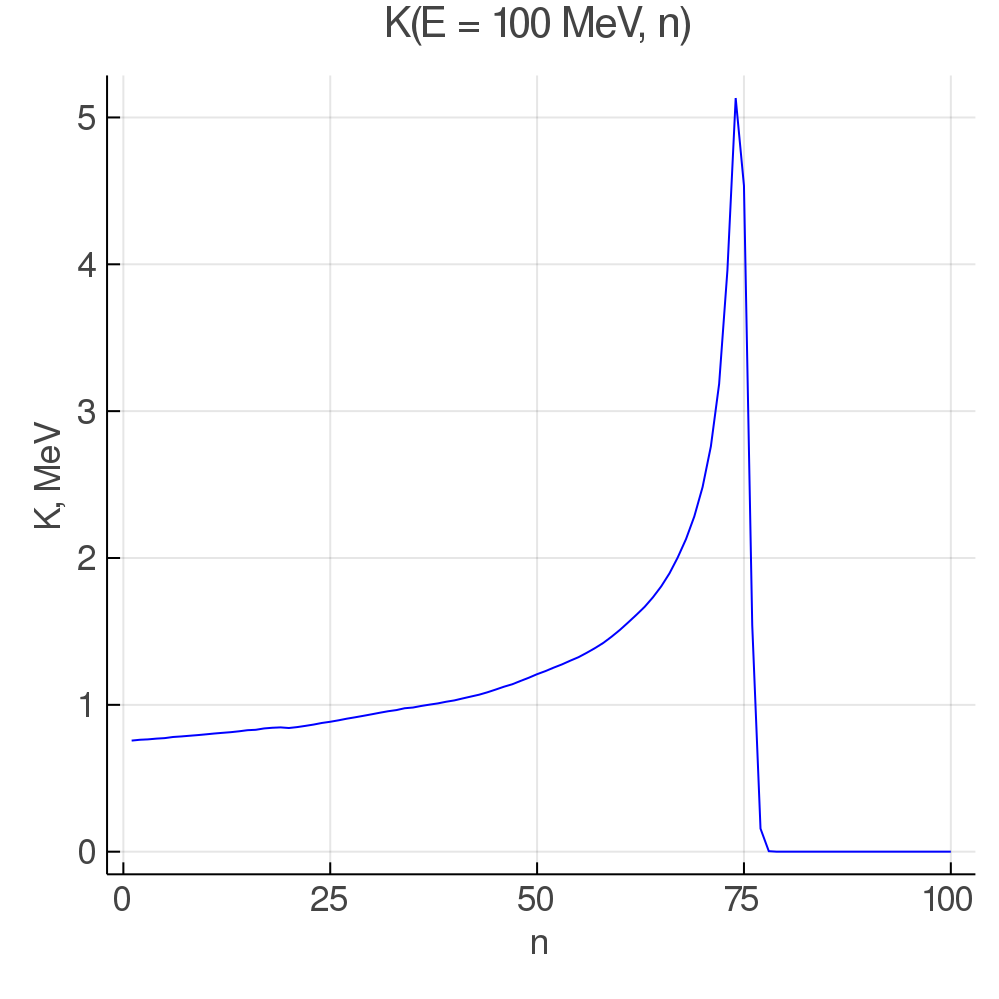
\includegraphics[width=\textwidth]{img/K.png}}
    \caption{Функция отклика детектора из 100 шайб по 1 мм толщиной для протона с энергией $E = 100$ MeV.}
    \label{K}
\end{minipage}
\hfill
\begin{minipage}[h]{0.45\linewidth}
\center{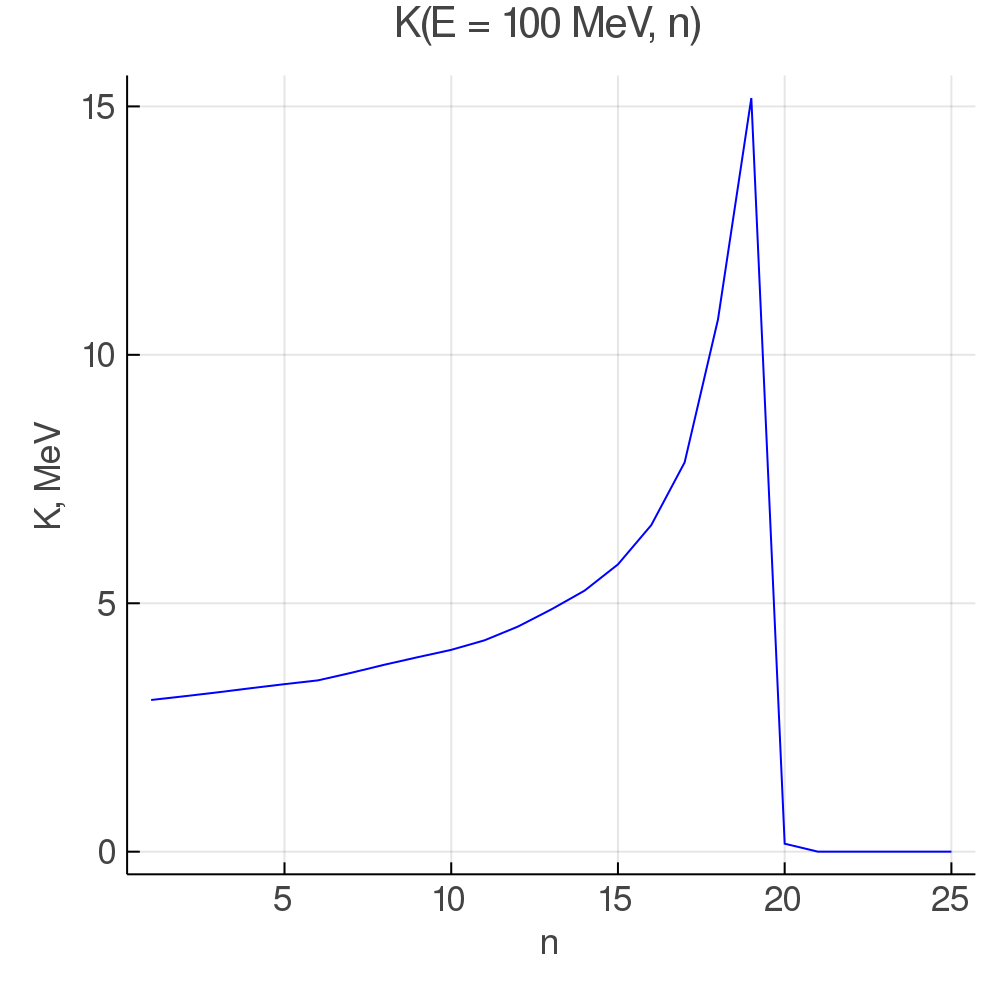
\includegraphics[width=\textwidth]{img/K_25.png}}
    \caption{Функция отклика детектора из 25 шайб по 4 мм толщиной для протона с энергией $E = 100$ MeV.}
    \label{K_25}
\end{minipage}
\end{figure}


Если попробовать напрямую решить матричное уравнение \ref{matrix_eq}, то получим негладкие зашумленные решения в обоих случаях (Рис. \ref{simple_solution}, \ref{simple_solution_25}). Среднее отклонение от реального спектра составляет $700\%$ и $14\%$ для 100 и 25 шайб соответственно.

\begin{figure}[h]
\begin{minipage}[h]{0.5\linewidth}
    \center{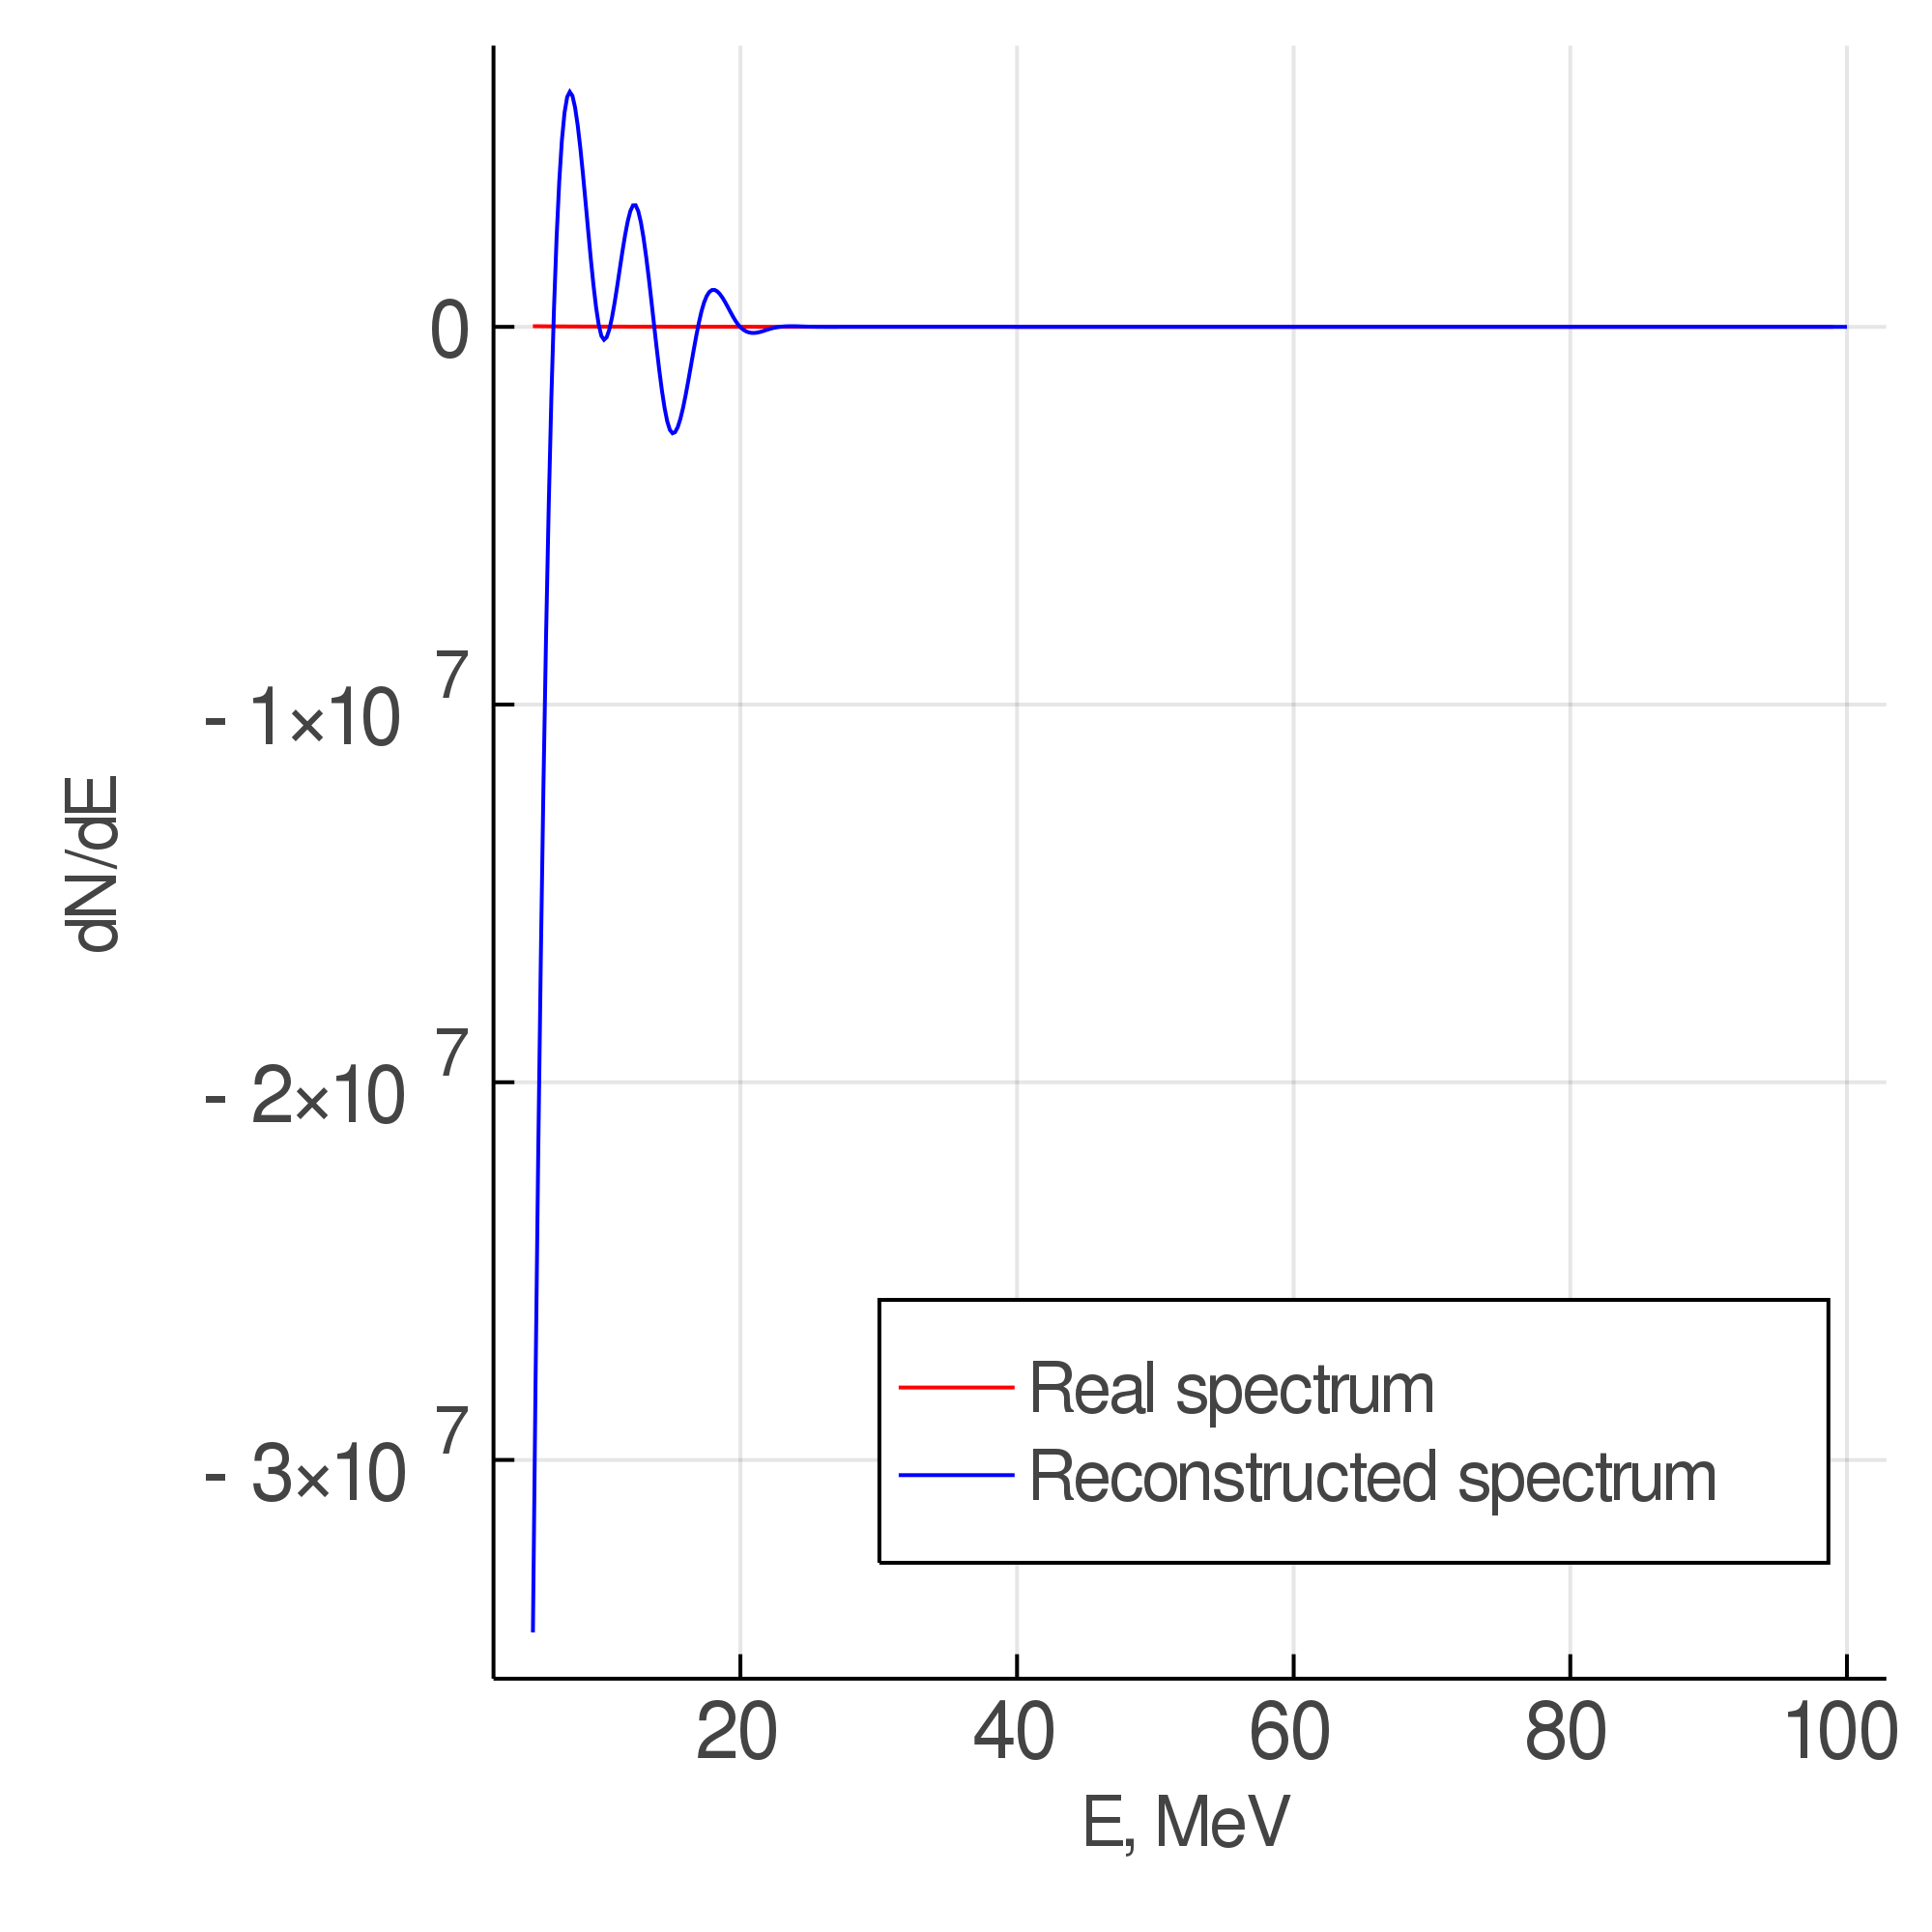
\includegraphics[width=\textwidth]{new_pic/matrix_solution.png}}
    \caption{Прямое решение матричного уравнения для детектора из 100 шайб.}
    \label{simple_solution}
\end{minipage}
\hfill
\begin{minipage}[h]{0.5\linewidth}
    \center{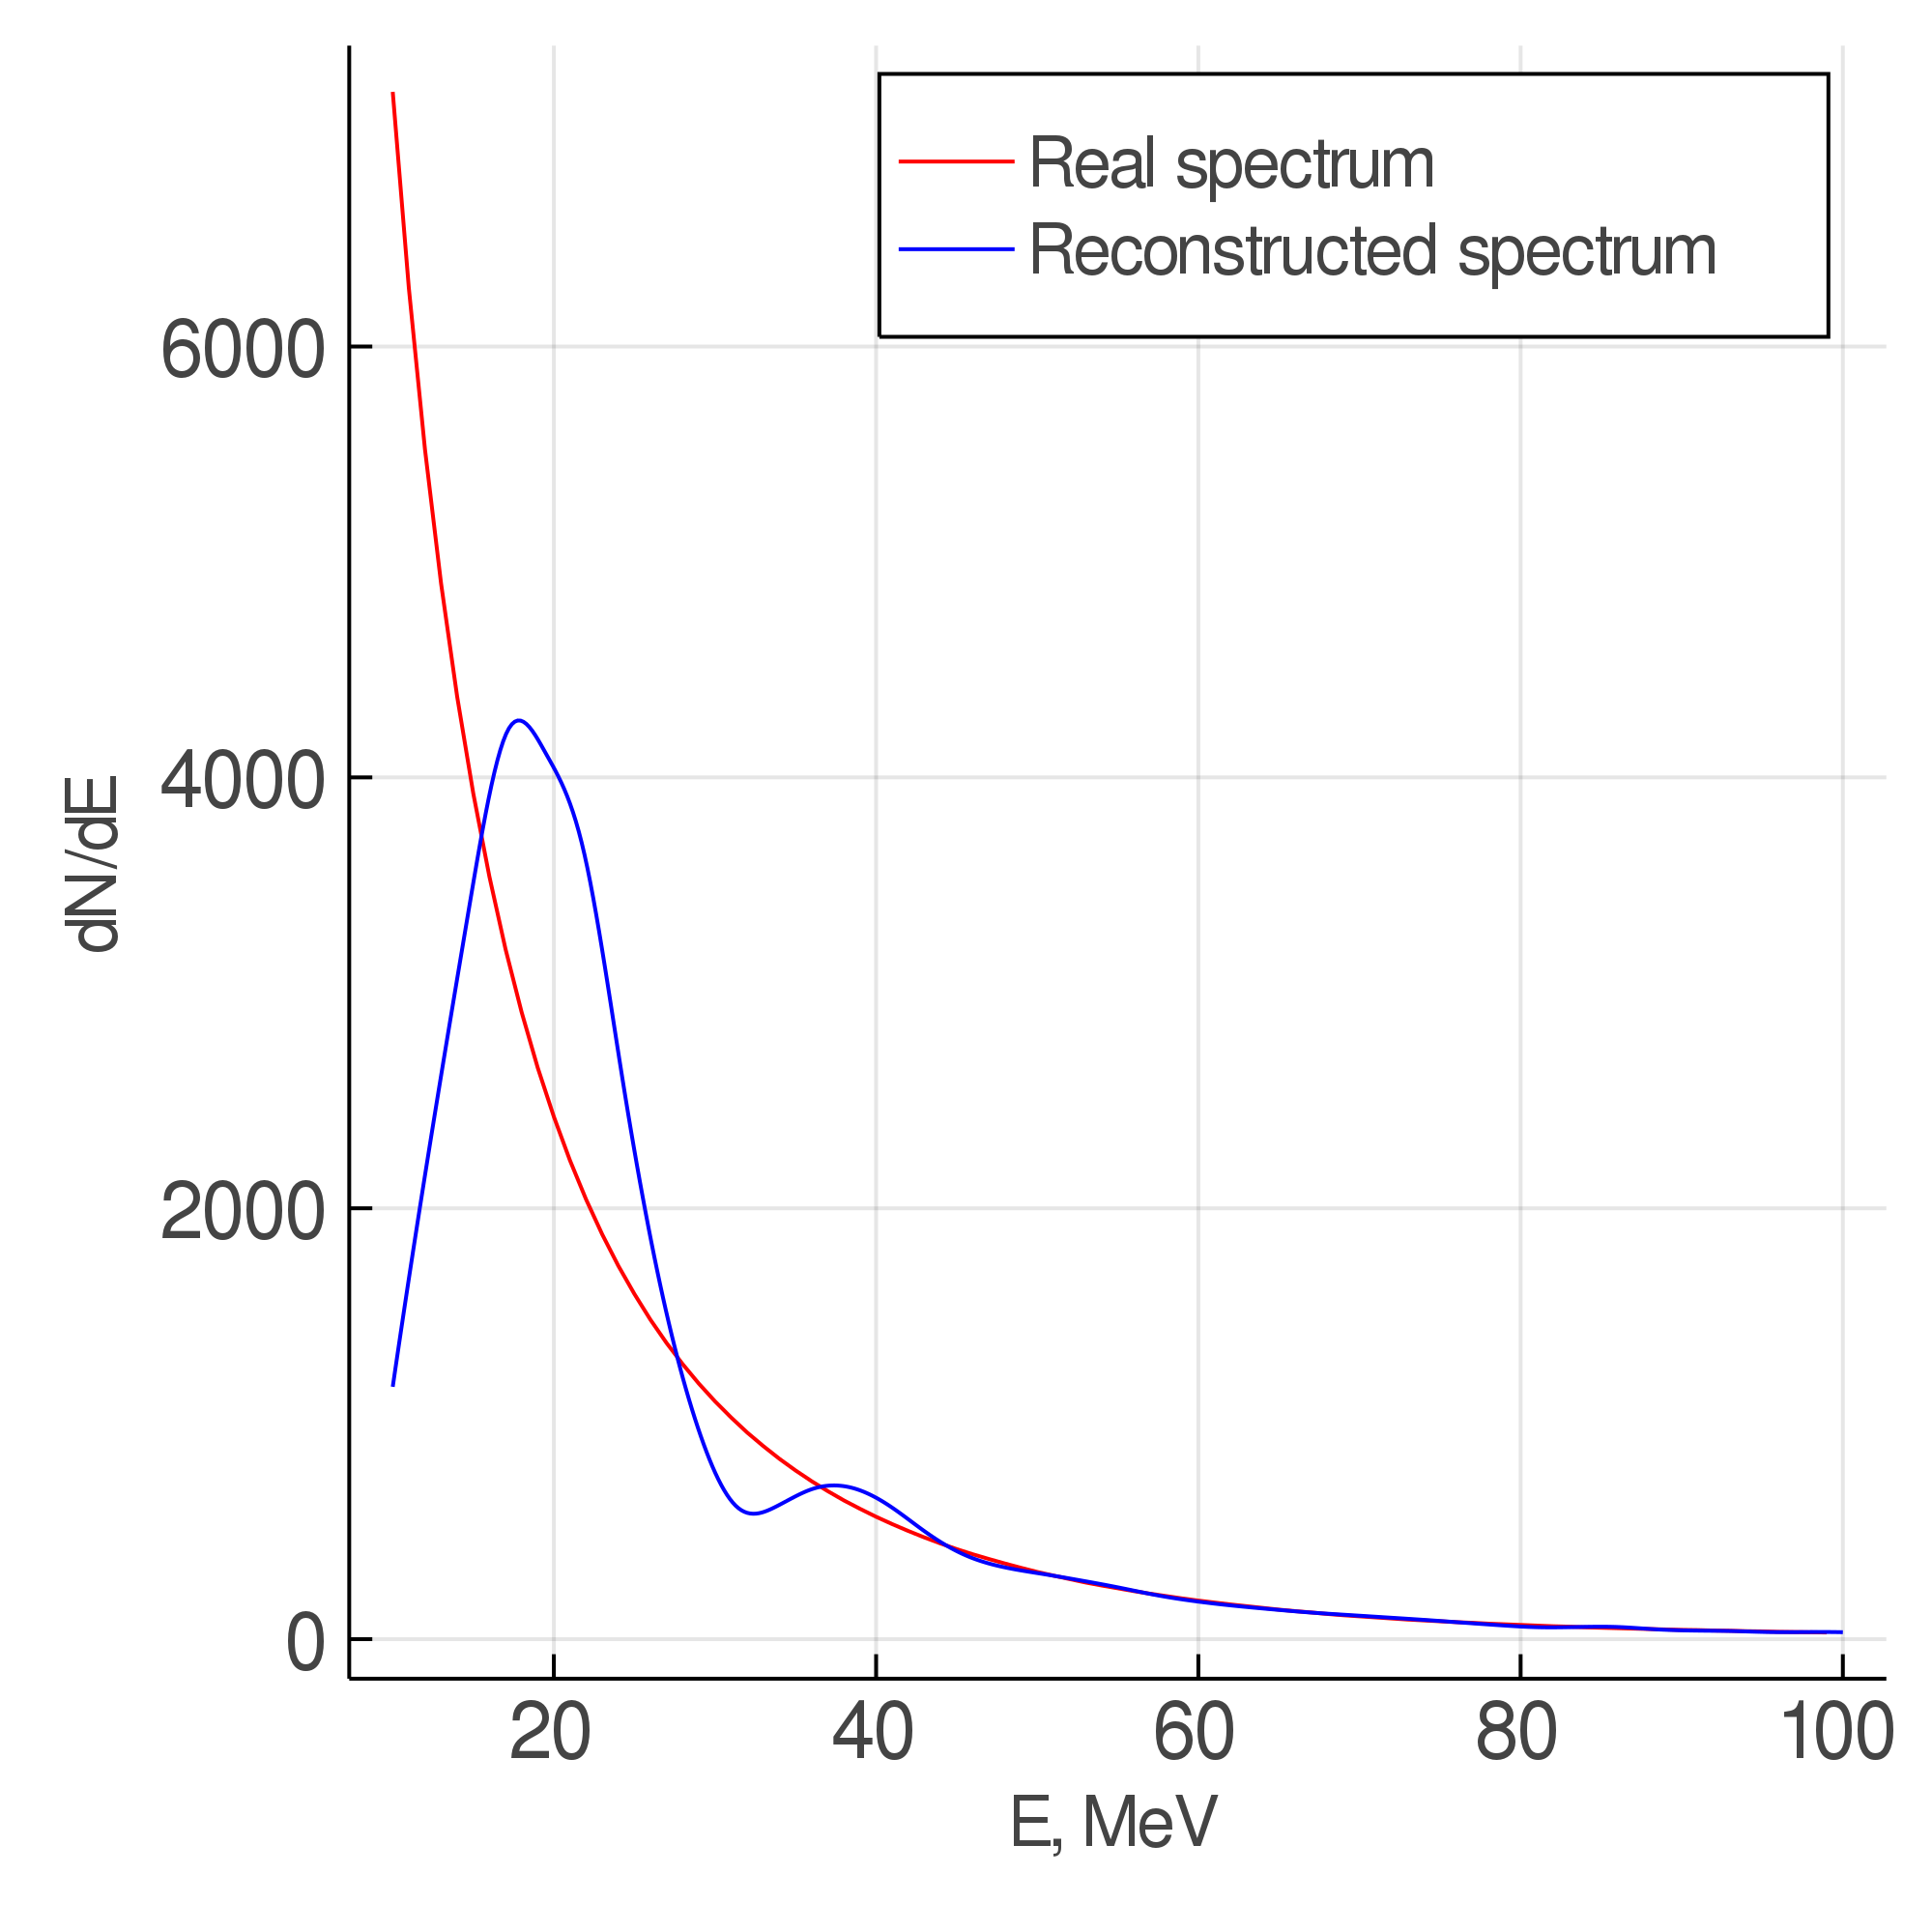
\includegraphics[width=\textwidth]{new_pic/matrix_solution_25.png}}
    \caption{Прямое решение матричного уравнения для детектора из 25 шайб.}
    \label{simple_solution_25}
\end{minipage}
\end{figure}

Выберем базис, состоящий из кубических сплайнов, количество функций - $n=60$.
\begin{minted}{julia}
basis = CubicSplineBasis(a, b, n, (nothing, "dirichlet"));
\end{minted}
В качестве априорной информации возьмем гладкость искомой функции. Для этого посчитаем матрицу средних значений вторых производных:
\begin{minted}{julia}
omegas = [omega(basis, 2)]
\end{minted}
В качестве параметра регуляризации $\alpha$ выберем наиболее вероятный. Он будет определяться с помощью пакета BAT.jl.
\begin{minted}{julia}
alphas = ArgmaxBAT()
\end{minted}
Граничные условия ставить не будем:
\begin{minted}{julia}
phi_bounds = PhiBounds()
\end{minted}
Будем считать, что измеренная величина $f$ имеет распределение Пуассона, которое в пределе стремится к распределению Гаусса: $\delta f = \sqrt{f}$. То есть, возможно найти аналитическое решение.
\begin{minted}{julia}
algo = Analytically()
\end{minted}
Найдем решение:
\begin{minted}{julia}
result = solve(
    basis,
    f,
    delta_f,
    K,
    measurement_points,
    algo,
    alphas,
    omegas
    phi_bounds,
    )
\end{minted}


На Рис. \ref{solution_cont} представлено восстановление спектра с использованием детектора из 100 шайб (диапазон энергий протонов - от 5 до 100 МэВ), на Рис. \ref{solution_25_cont} представлено восстановление спектра с использованием детектора из 25 шайб (диапазон энергий протонов - от 10 до 100 МэВ). Средняя ошибка восстановления спектра составляет $7\%$.

\begin{figure}[h]
\begin{minipage}[h]{0.45\linewidth}
        \center{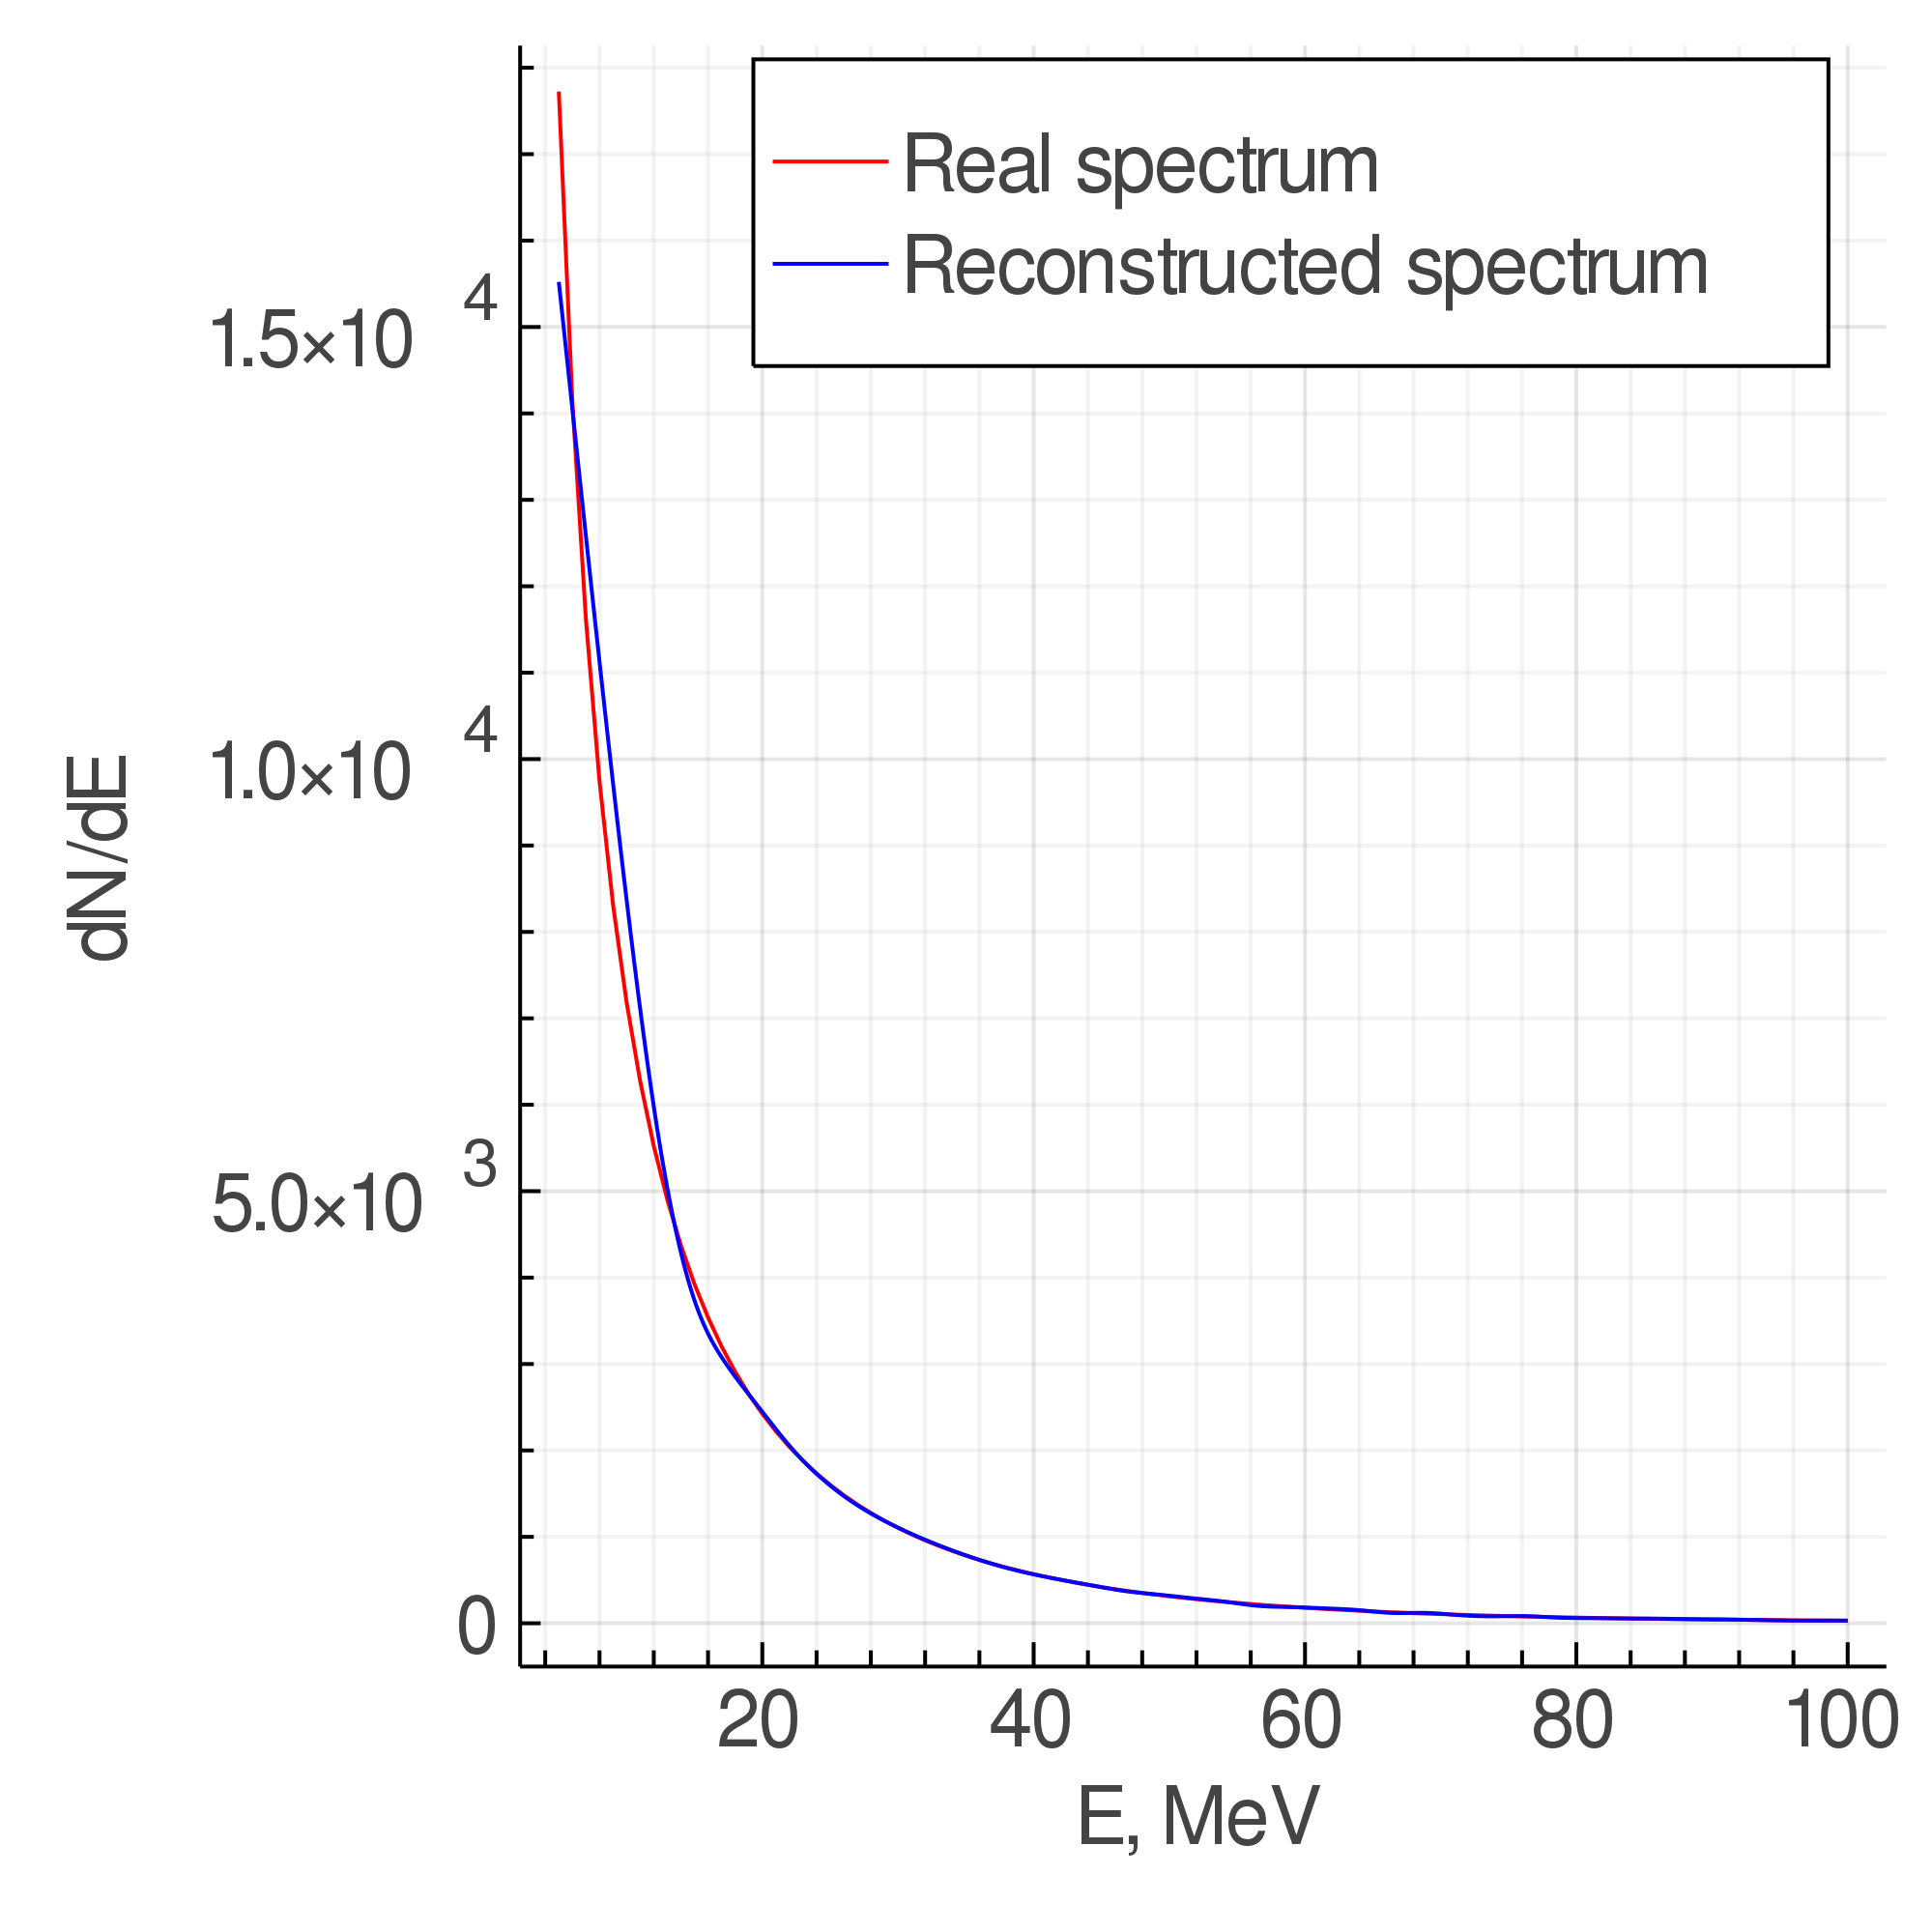
\includegraphics[width=\textwidth]{new_pic/reconstructed_from_5.png}}
    \caption{Восстановленный спектр для базиса из 60 кубических сплайнов и детектора из 100 шайб.}
    \label{solution_cont}
\end{minipage}
\hfill
\begin{minipage}[h]{0.45\linewidth}
        \center{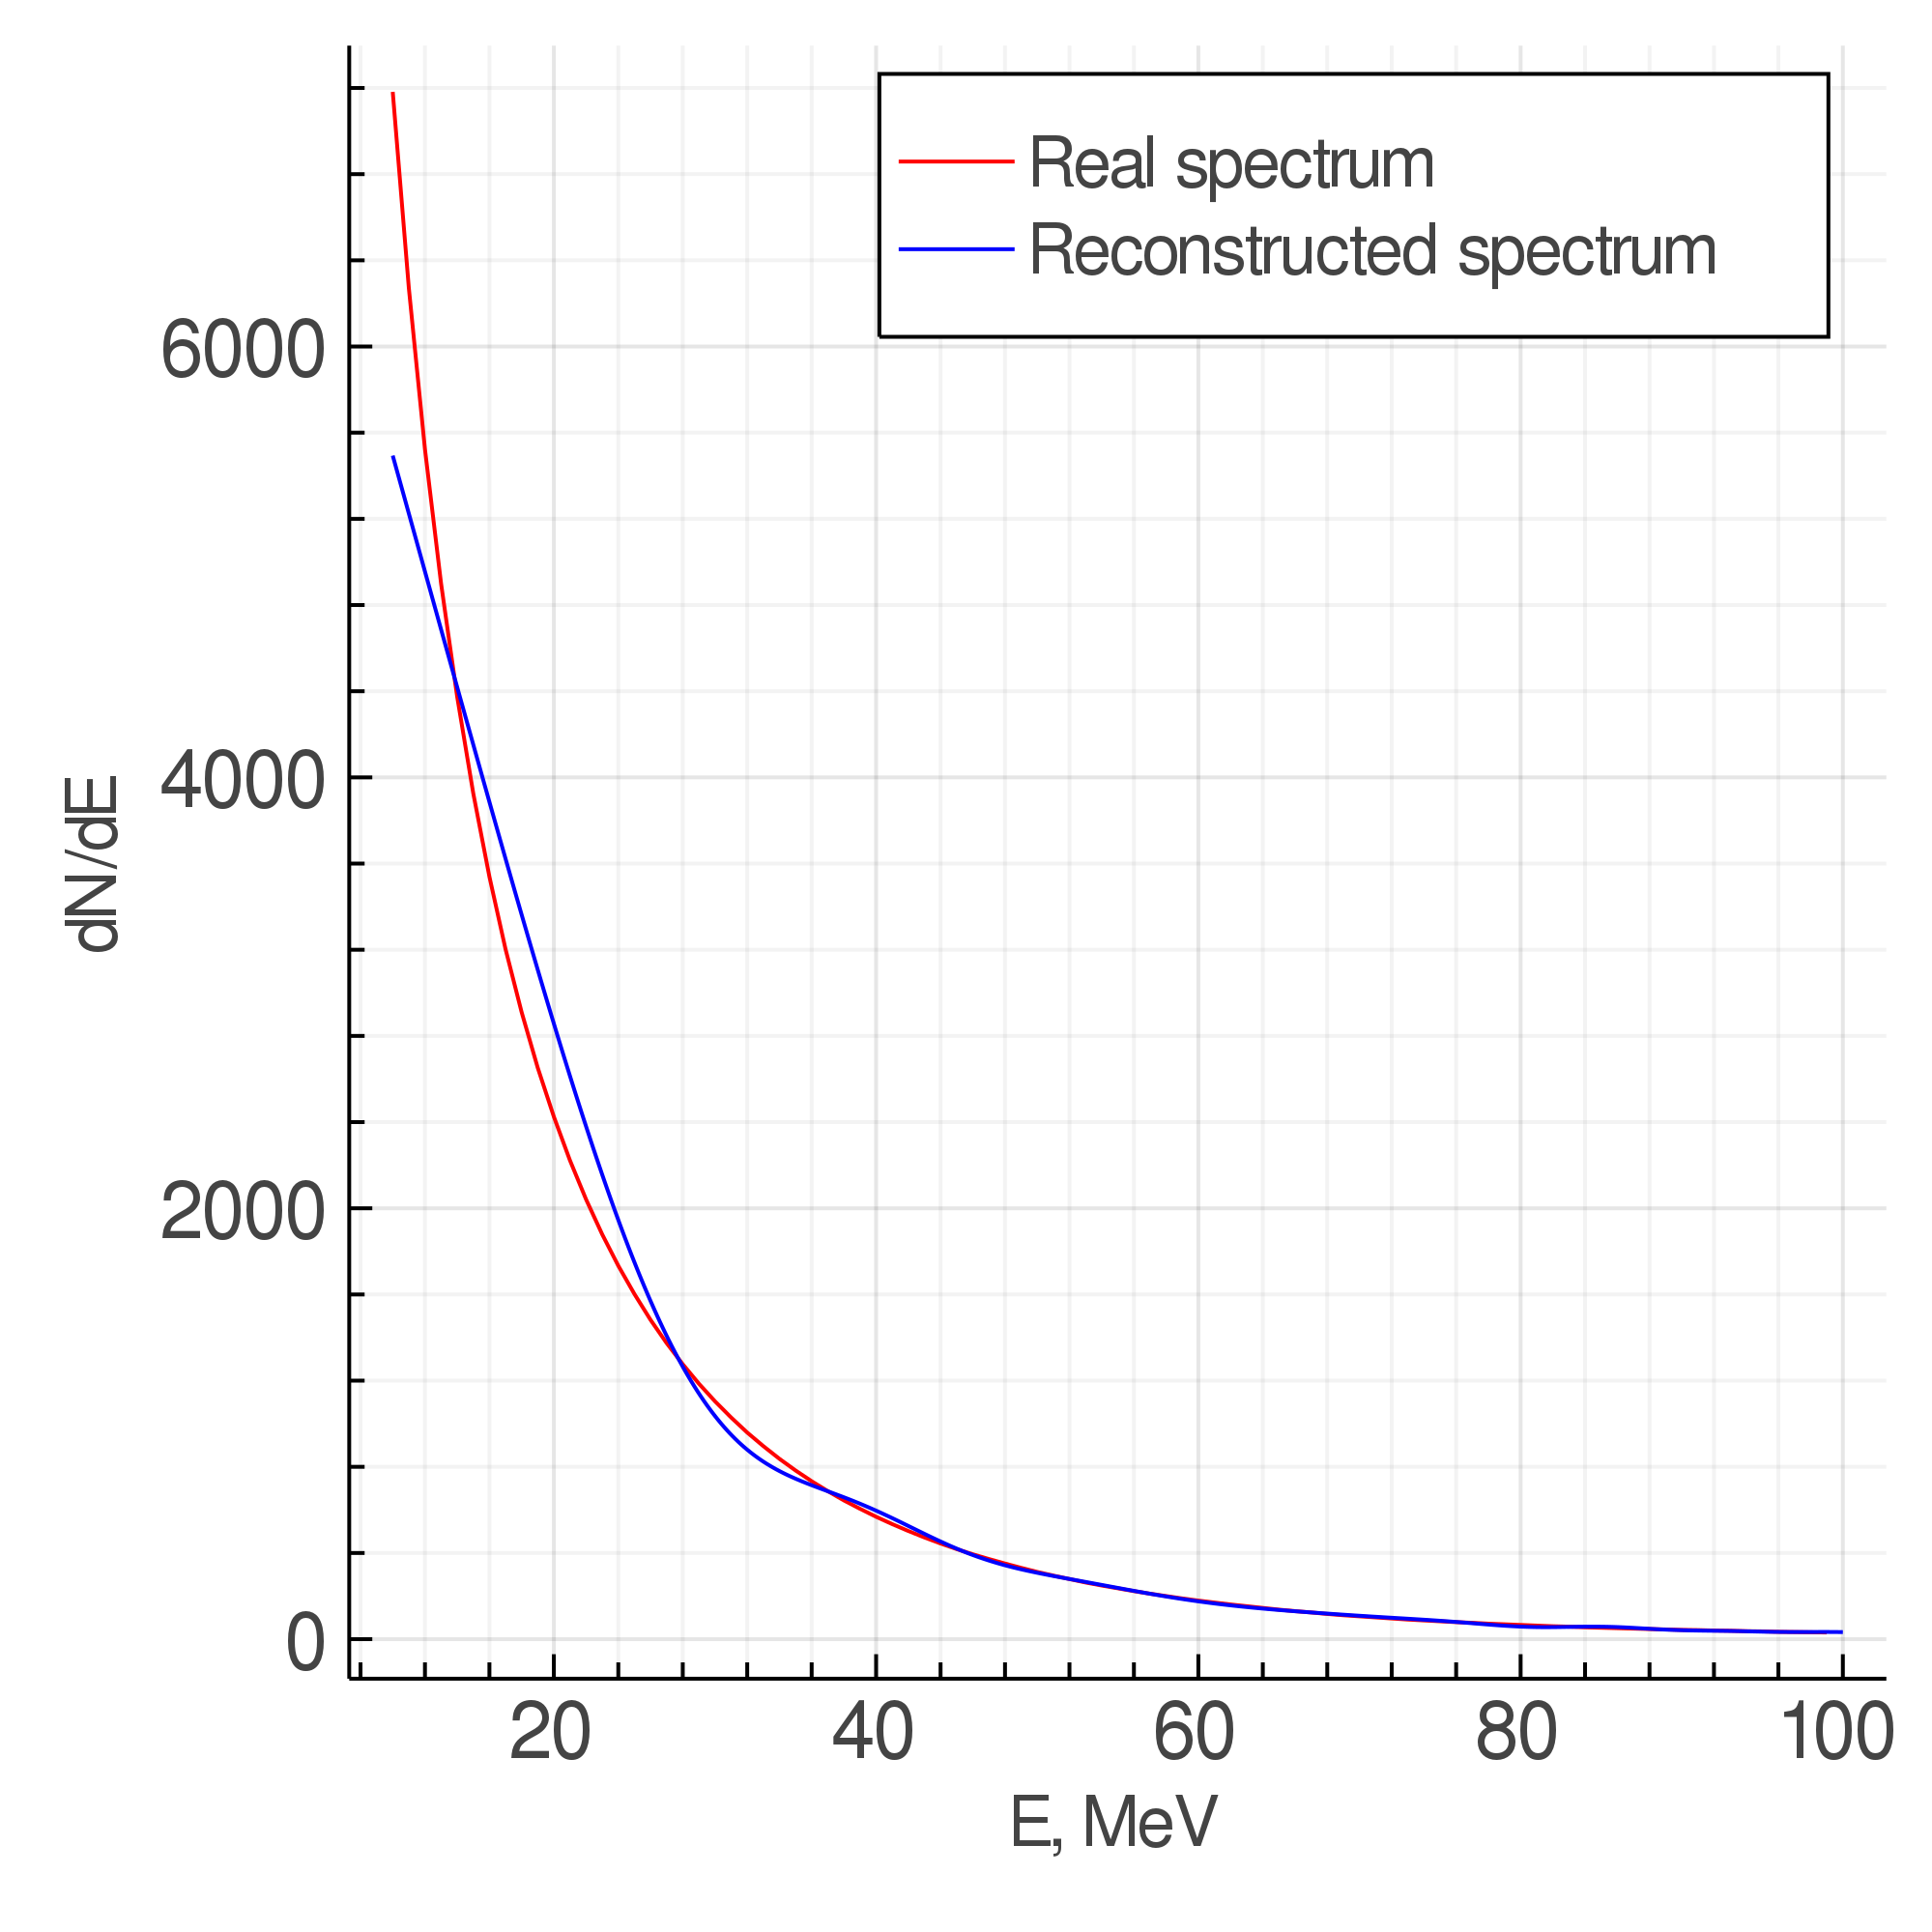
\includegraphics[width=\textwidth]{new_pic/reconstructed_25_from_10.png}}
    \caption{Восстановленный спектр для базиса из 60 кубических сплайнов и детектора из 25 шайб.}
    \label{solution_25_cont}
\end{minipage}
\end{figure}


Аналогичным образом восстановление было проведено для других угловых распределений (Рис. \ref{uniform}, \ref{gaussian}).

\begin{figure}[h]
\begin{minipage}[h]{0.45\linewidth}
    \center{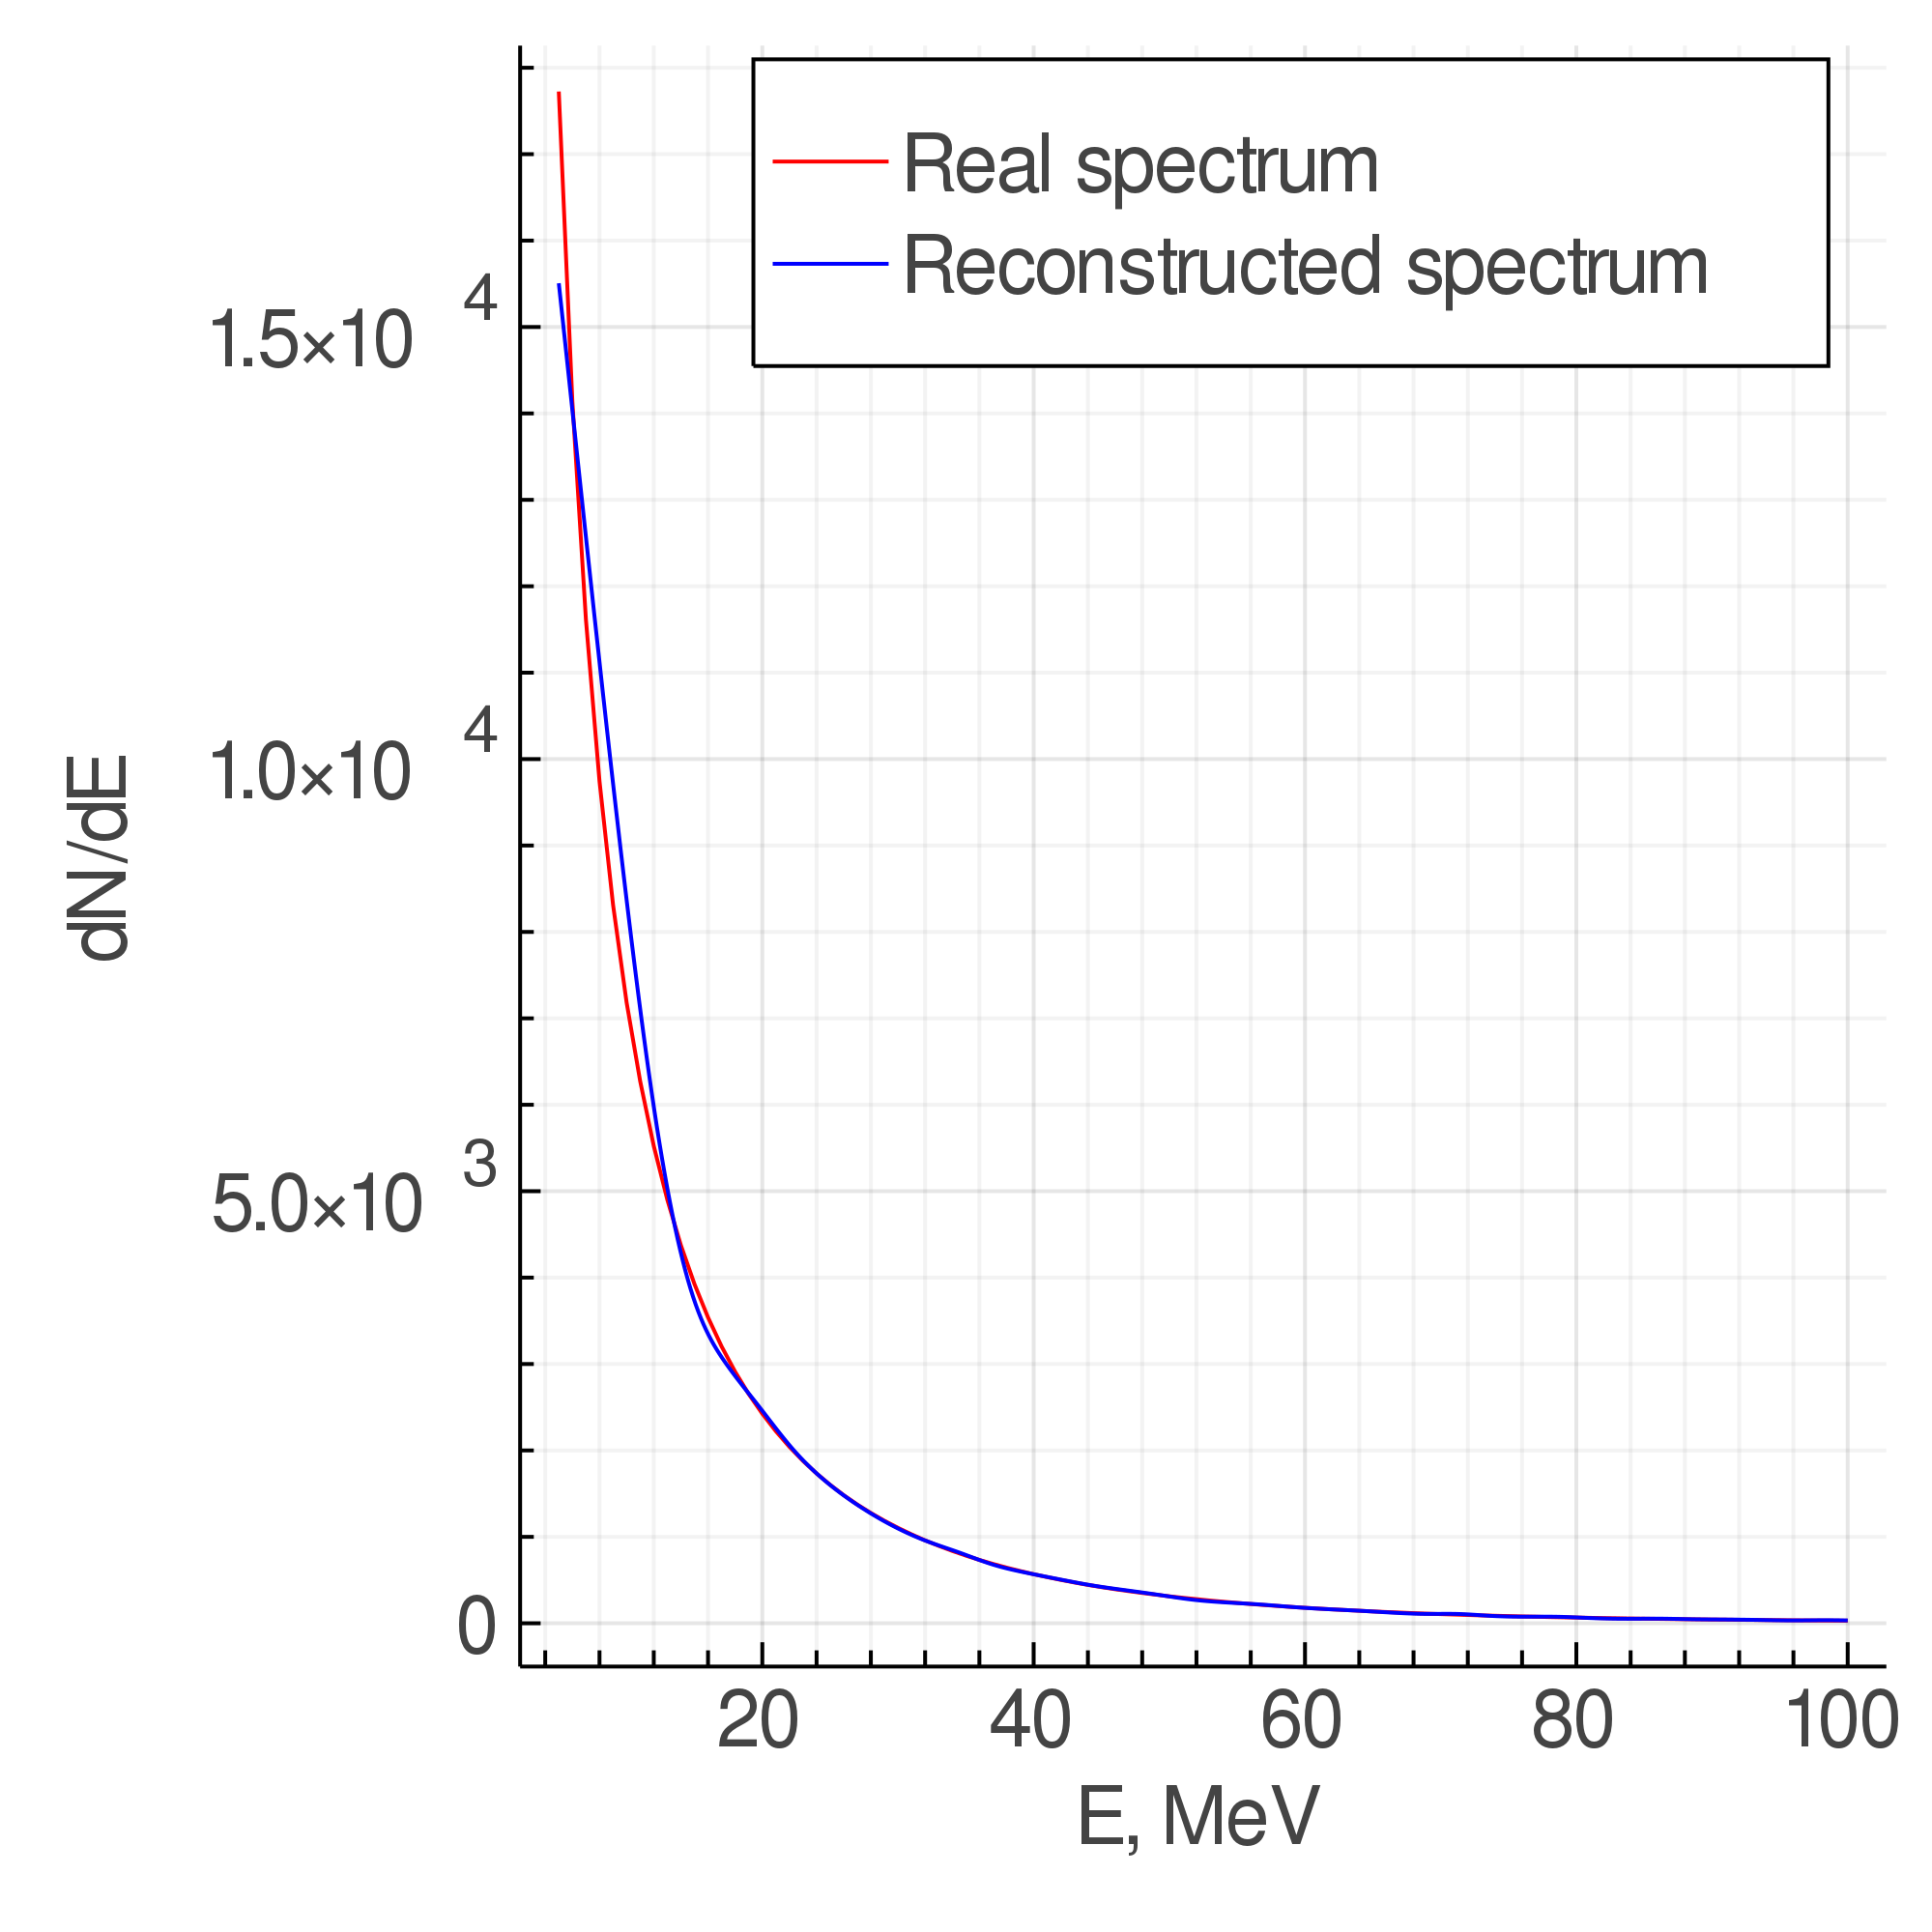
\includegraphics[width=\textwidth]{new_pic/reconstructed_from_5_uniform15.png}}
    \caption{Восстановленный спектр для базиса из 60 кубических сплайнов и детектора из 100 шайб для равномерного распределения частиц по углу от $0^\circ$ до $15^\circ$.}
    \label{uniform}
\end{minipage}
\hfill
\begin{minipage}[h]{0.45\linewidth}
\center{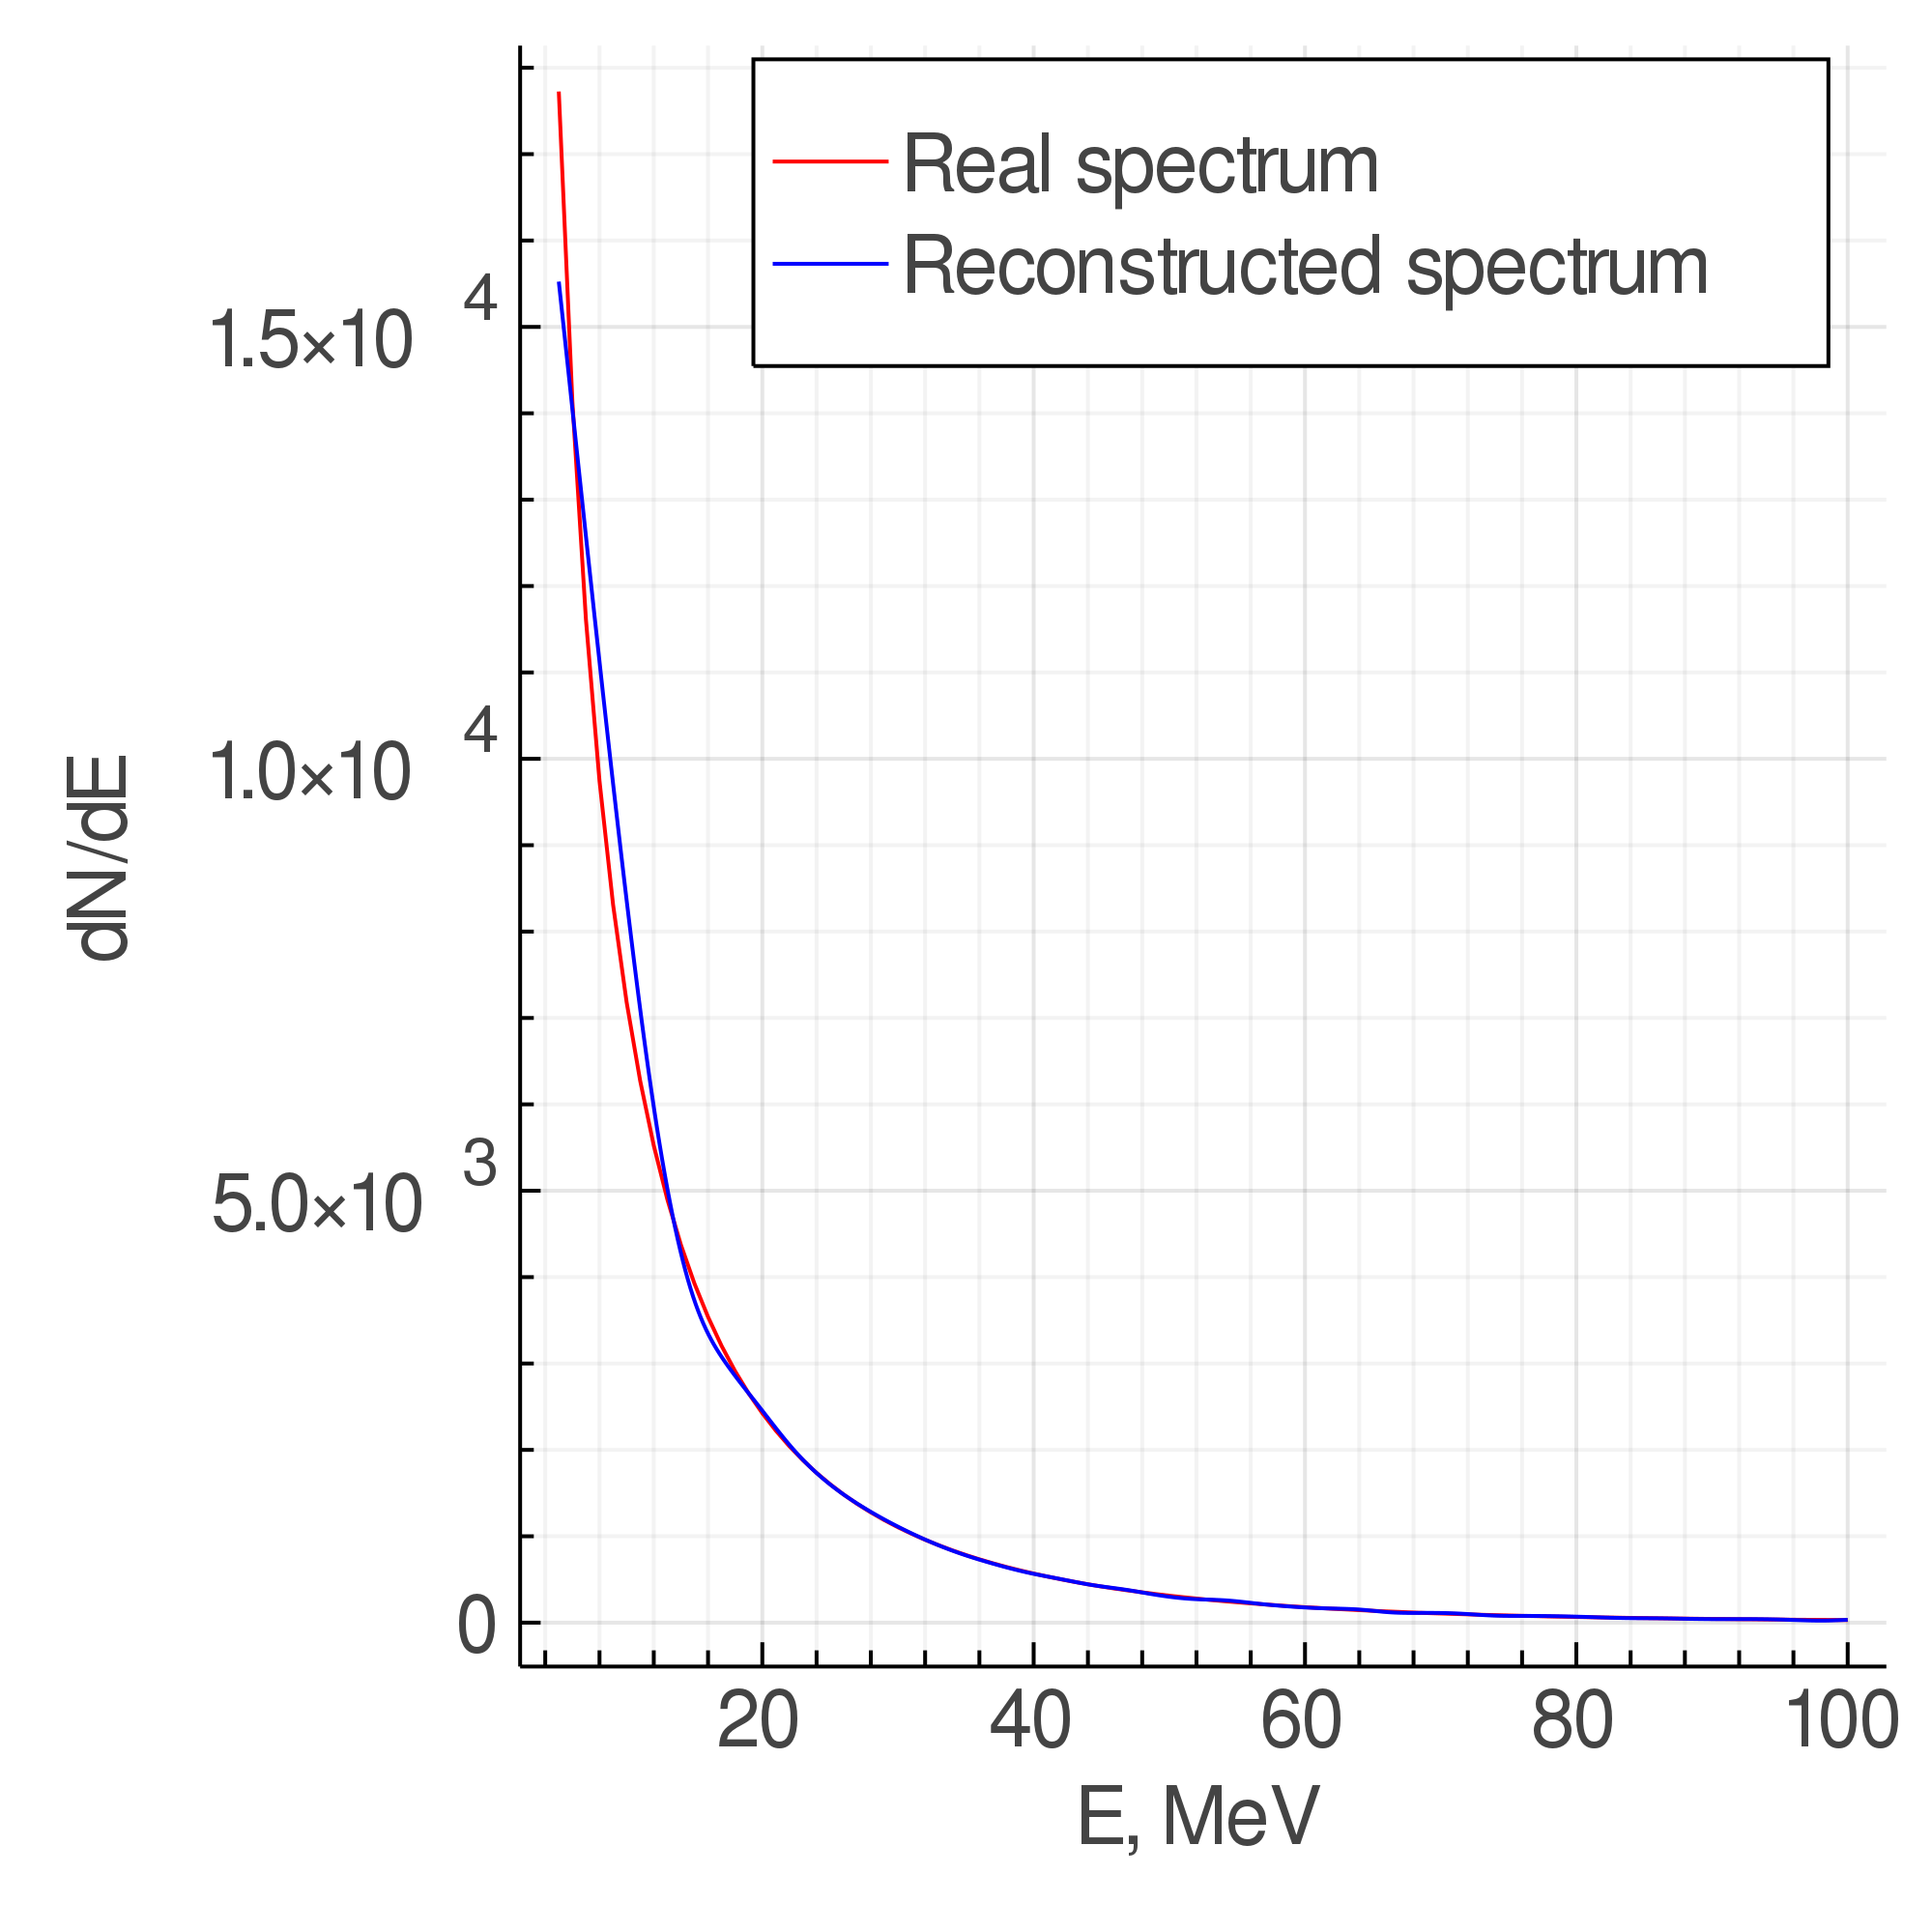
\includegraphics[width=\textwidth]{new_pic/reconstructed_from_5_gaussian.png}}
    \caption{Восстановленный спектр для базиса из 60 кубических сплайнов и детектора из 100 шайб для нормального распределения частиц по углу с матожиданием $\mu = 0^\circ$ и дисперсией $\sigma = 5^\circ$.}
    \label{gaussian}
\end{minipage}
\end{figure}


Таким образом, для всех опробованных распределений по углу, конфигураций детектора и числа базисных функций получилась точность лучше 10$\%$.



\clearpage

\section{Заключение}
Целью настоящей работы являлось восстановление энергетического спектра протонов космического излучения. Для этого был разработан пакет программного кода на языке программирования Julia. Пакет позволяет:
\begin{itemize}
    \item осуществлять восстановление спектров путем разложения искомой функции по набору различных функциональных базисов
    \item использовать различную априорную информацию о функции
    \item ставить граничные условия на коэффициенты при базисных функциях
    \item представлять результаты в удобном для анализа и понимания виде
\end{itemize}
Данный пакет был применен для обработки данных, смоделированных с помощью Geant4. В результате удалось восстановить спектр протонов космического излучения со средней ошибкой менее $7\%$.

\textit{
Настоящая работа выполнена в группе методики ядерно-физических экспериментов при ИЯИ РАН и МФТИ. Я выражаю благодарность своему научному руководителю Александру Нозику за за постановку интересной задачи, активное руководство, а также проявленное терпение и внимание. Я также благодарна Оливеру Шульцу за помощь в освоении нового для меня языка программирования Julia и Михаилу Зелёному за ценные советы по работе с Geant4 и помощь с моделированием отклика детектора и энерговыделений.}
\clearpage

\section{Приложения}
\subsection{Явный вид априорного распределения}
~~~~Для нахождения явного вида априорного распределения нужно решить следующую систему уравнений:
\begin{equation*}
 \begin{cases}
   \alpha \int (\vec{\varphi}, \Omega \vec{\varphi}) P_{\alpha}(\vec{\varphi}) d\vec{\varphi} = 1\\
   \int P_{\alpha}(\vec{\varphi}) \ln{P_{\alpha}(\vec{\varphi})}d \vec{\varphi} \rightarrow \min{}
 \end{cases}
\end{equation*}
Воспользуемся методом множителей Лагранжа для решения задачи нахождения условного экстремума:
\begin{equation}
    L(\vec{\varphi}, \lambda) = P(\vec{\varphi}) \ln{P(\vec{\varphi})} + \lambda (\vec{\varphi}, \Omega \vec{\varphi}) P(\vec{\varphi})
\end{equation}

\begin{equation}
    \frac{\partial L}{\partial \vec{\varphi}} = P'(\vec{\varphi}) (1 + \ln{P(\vec{\varphi})} + \lambda (\vec{\varphi}, \Omega \vec{\varphi})) = \vec{0}
\end{equation}

\begin{equation}
    \alpha \int (\vec{\varphi}, \Omega \vec{\varphi}) P(\vec{\varphi}) d\vec{\varphi} = 1
\end{equation}

\begin{equation}
    P_{\alpha}(\vec{\varphi}) \sim exp(-\frac{1}{2} (\vec{\varphi}, \alpha \Omega \vec{\varphi}))
\end{equation}

Нормировку можно найти из сходства с нормальным распределением.
\begin{equation}
    P_{\alpha}(\vec{\varphi}) = \frac{\det{\alpha \Omega}}{(2\pi)^{M/2}} exp(-\frac{1}{2} (\vec{\varphi}, \alpha \Omega \vec{\varphi}))
\end{equation}

\subsection{Аналитическое решение в случае нормального распределения измеряемой величины}
По формуле Байеса:
\begin{equation}
    P(\vec{\varphi} | \vec{f}) \sim P(\vec{\varphi}) P(\vec{f} | \vec{\varphi})
\end{equation}

\begin{equation}
    P(\vec{f} | \varphi) = \frac{1}{(2\pi)^{M/2} \sqrt{\det{\Sigma}}}\exp{-\frac{1}{2}(\vec{f} - K \vec{\varphi})^T \Sigma^{-1} (\vec{f} - K \vec{\varphi})}
\end{equation}

\begin{equation}
    P_{\alpha}(\vec{\varphi}) = \frac{\det{\alpha \Omega}}{(2\pi)^{N/2}} exp(-\frac{1}{2} (\vec{\varphi}, \alpha \Omega \vec{\varphi}))
\end{equation}

\begin{equation}
    P(\vec{\varphi} | \vec{f}) \sim exp(-\frac{1}{2}(\vec{f}^T \Sigma^{-1} \vec{f} - \vec{f}^T \Sigma^{-1} K \vec{\varphi} -
\vec{\varphi}^T K^T \Sigma^{-1} \vec{f} + \vec{\varphi}^T K^T
\Sigma^{-1} K \vec{\varphi} + \vec{\varphi}^T \alpha \Omega
\vec{\varphi}))
\end{equation}

\begin{equation}
    P(\vec{\varphi} | \vec{f}) \sim exp(-\frac{1}{2}\vec{\varphi}^T(\alpha \Omega + K^T \Sigma^{-1} \vec{f})\vec{\varphi} + (\vec{f} \Sigma^{-1} K)\vec{\varphi}) \sim exp(-\frac{1}{1}\vec{\varphi}^T A \vec{\varphi} + \vec{b}^T \vec{\varphi})
\end{equation}

Получили нормальное распределение общего вида. Его матожидание:
\begin{equation}
    \vec{\varphi}_{opt} = A^{-1} b = (K^T \Sigma^{-1}K + \alpha \Omega)^{-1} K^T \Sigma^{-1T} \vec{f}
\end{equation}

Его матрица ковариаций:
\begin{equation}
    cov = A^{-1} = (K^T \Sigma^{-1} K + \alpha \Omega)^{-1}
\end{equation}

\subsection{Базисы}
\begin{enumerate}
    \item Фурье-базис\newline
Вид функций: $\{1, \sin{x}, \cos{x}, ..., \sin{nx}, \cos{nx}\}$ \newline
График функций представлен на Рис. \ref{basis_fourier}

\begin{figure}[h!]
    \center{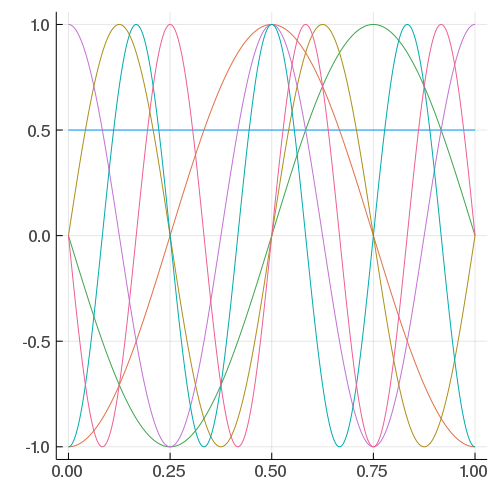
\includegraphics[width=0.6\textwidth]{img/basis_fourier.png}}
    \caption{Фурье-базис.}
    \label{basis_fourier}
\end{figure}

    \item Базис из полиномов Лежандра\newline
Вид функций: $P_n(x) = \frac{1}{2^n n!} \frac{d^n}{dx^n} (z^2 - 1)^n$ \newline
График функций представлен на Рис. \ref{basis_legendre}

\begin{figure}[h!]
    \center{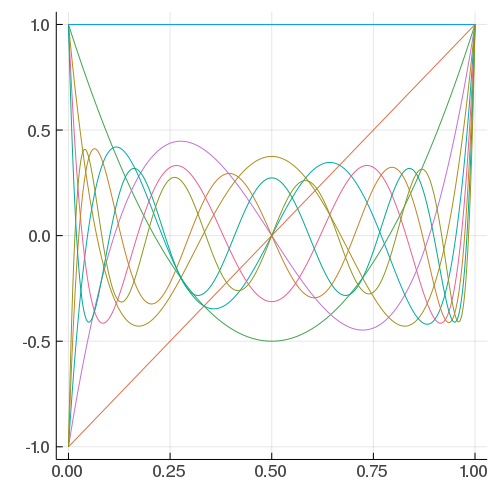
\includegraphics[width=0.6\textwidth]{img/basis_legendre.png}}
    \caption{Базис из полиномов Лежандра.}
    \label{basis_legendre}
\end{figure}

    \item Базис из полиномов Бернштейна\newline
Вид функций: $B_{k, n}(x) = C_n^k x^k (1-x)^{n-k}$ \newline
График функций представлен на Рис. \ref{basis_bernstein}

\begin{figure}[h!]
    \center{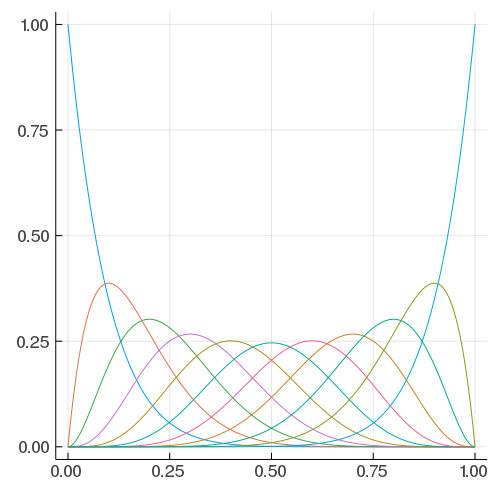
\includegraphics[width=0.6\textwidth]{img/basis_bernstein.png}}
    \caption{Базис из полиномов Бернштейна.}
    \label{basis_bernstein}
\end{figure}

    \item Базис из кубических сплайнов\newline
Вид функций: пусть дан набор узлов $\{x_i\}_{i=0}^I$
\begin{equation}
    B_{i, 1}(x) = 
    \begin{cases}
    1, & x_i \leq x < x_{i+1}\\
    0, & otherwise
    \end{cases}
\end{equation}

\begin{equation}
    B_{i, k+1}(x) = \frac{x - x_i}{x_{i+k} - x_i} B_{i, k}(x) + \frac{x_{i+k+1} - x}{x_{i+k+1} - x_{i+1}} B_{i+1, k}(x)
\end{equation}

График функций представлен на Рис. \ref{basis_cubic}
\end{enumerate}

\begin{figure}[h!]
    \center{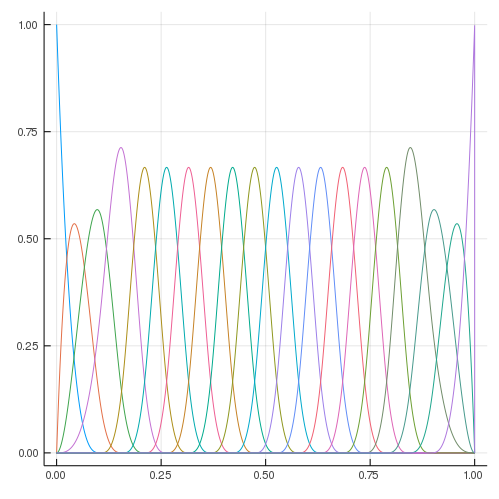
\includegraphics[width=0.6\textwidth]{img/basis_cubic.png}}
    \caption{Базис из кубических сплайнов.}
    \label{basis_cubic}
\end{figure}

\clearpage

\printbibliography[
heading=bibintoc,
title={Список литературы}
]

\end{document}
